% TODO: Clean or remove table about references tab:tabApp2.1
% TODO: maxN nomenclature -> extended LH dataset
%************************************************
\chapter[Appendix 2: Chapter 2 - Supplementary materials]{Appendix 2: Chapter 2
- Supplementary materials}\label{ch:Appendix2.1}
%************************************************

\renewcommand{\thefigure}{A.2.\arabic{figure}}
\setcounter{figure}{0}

\renewcommand{\thetable}{A.2.\arabic{table}}
\setcounter{table}{0}

\section*{Supplementary tables}

% \afterpage{
% \clearpage% Flush earlier floats (otherwise order might not be correct)
% \begin{landscape}
% 
% \begin{longtable}[]{p{2cm}p{2cm}p{2cm}p{2cm}p{2cm}p{2cm}p{2cm}p{2cm}p{2cm}p{2cm}p{2cm}p{2cm}}
% \centering
% \caption[Previous works]{Articles describing life history axes.}
% \label{tab:tabApp2.1}
% % \begin{tabular}{@{}llllllllllll@{}}
% \toprule
% \textbf{Work}                                                                                          & \textbf{Methods}                                                                                              & \textbf{Phylogenetic treatment}                                             & \textbf{Body size}                                                                                                                     & \textbf{Traits}                                                                                                                                                                                                                                                                                                                                                                                                                                                                                                                                                                                                                                                & \textbf{Transformations}                    & \textbf{Axes}                                                                                                   & \textbf{N}                       & \textbf{group}       & \textbf{Fast-Slow}                                                                                                                                                                                                                                                                                                                                                                                                                                                                                                                                                                                                                                                                                                                                                                                                                                                                                                                                                                                     & \textbf{2on axis}                                                                                                                                                                                                                                                                                                                                                                                                                                                                                                                                                                                                                                                                                                                                                                                           & \textbf{comments}                                                                                                                                                                                                                                                                                                                                                                                                                                                                                                                                                                                                                                                                                                                                                                                                                                                                                                                                                                                                                                                                                                                                                             \\ \midrule
% Millar 1977                                                                                            &                                                                                                               &                                                                             &                                                                                                                                        &                                                                                                                                                                                                                                                                                                                                                                                                                                                                                                                                                                                                                                                                &                                             & Size                                                                                                            &                                  &                      &                                                                                                                                                                                                                                                                                                                                                                                                                                                                                                                                                                                                                                                                                                                                                                                                                                                                                                                                                                                                        &                                                                                                                                                                                                                                                                                                                                                                                                                                                                                                                                                                                                                                                                                                                                                                                                             &                                                                                                                                                                                                                                                                                                                                                                                                                                                                                                                                                                                                                                                                                                                                                                                                                                                                                                                                                                                                                                                                                                                                                                               \\
% Western 1979                                                                                           & linear regressions                                                                                            & Correlation by order with body size                                         &                                                                                                                                        & body weight (W), gestation time (g), age at first reproduction (a), life expectancy at birth (eo), life span (I) and birth rate (h). Age at first reproduction was taken as age at sexual maturity plus gestation time. Birth rate was taken as the percentage of young born each year to the whole population or a representative sample of it.                                                                                                                                                                                                                                                                     & log                                         & Size                                                                                                            &                                  & mammals              & \cellcolor[HTML]{F00}First order strategies: correlation of various life history processes with size                                                                                                                                                                                                                                                                                                                                                                                                                                                                                                                                                                                                                                                                                                                                                                                                                                                                                                   & second order strategies (r/K)                                                                                                                                                                                                                                                                                                                                                                                                                                                                                                                                                                                                                                                                                                                                                                               & Brain size                                                                                                                                                                                                                                                                                                                                                                                                                                                                                                                                                                                                                                                                                                                                                                                                                                                                                                                                                                                                                                                                                                                                                                    \\
% Eisenberg, J. F. 1981. The mammalian radiations. University of Chicago Press, Chicago.                 &                                                                                                               &                                                                             &                                                                                                                                        &                                                                                                                                                                                                                                                                                                                                                                                                                                                                                                                                                                                                                                                                &                                             &                                                                                                                 &                                  &                      &                                                                                                                                                                                                                                                                                                                                                                                                                                                                                                                                                                                                                                                                                                                                                                                                                                                                                                                                                                                                        &                                                                                                                                                                                                                                                                                                                                                                                                                                                                                                                                                                                                                                                                                                                                                                                                             &                                                                                                                                                                                                                                                                                                                                                                                                                                                                                                                                                                                                                                                                                                                                                                                                                                                                                                                                                                                                                                                                                                                                                                               \\
% Peters 1983                                                                                            &                                                                                                               &                                                                             &                                                                                                                                        &                                                                                                                                                                                                                                                                                                                                                                                                                                                                                                                                                                                                                                                                &                                             & Size                                                                                                            &                                  &                      &                                                                                                                                                                                                                                                                                                                                                                                                                                                                                                                                                                                                                                                                                                                                                                                                                                                                                                                                                                                                        &                                                                                                                                                                                                                                                                                                                                                                                                                                                                                                                                                                                                                                                                                                                                                                                                             &                                                                                                                                                                                                                                                                                                                                                                                                                                                                                                                                                                                                                                                                                                                                                                                                                                                                                                                                                                                                                                                                                                                                                                               \\
% Millar and Zammuto 1983                                                                                &                                                                                                               &                                                                             &                                                                                                                                        &                                                                                                                                                                                                                                                                                                                                                                                                                                                                                                                                                                                                                                                                &                                             & Size                                                                                                            &                                  &                      &                                                                                                                                                                                                                                                                                                                                                                                                                                                                                                                                                                                                                                                                                                                                                                                                                                                                                                                                                                                                        &                                                                                                                                                                                                                                                                                                                                                                                                                                                                                                                                                                                                                                                                                                                                                                                                             &                                                                                                                                                                                                                                                                                                                                                                                                                                                                                                                                                                                                                                                                                                                                                                                                                                                                                                                                                                                                                                                                                                                                                                               \\
% Stearns1983a                                                                                           & PCA and cluster analysis                                                                                      & Control for family and order                                                & Raw and residuals                                                                                                                      & adult mass, longevity, gestation period, age at eye opening, weight of offspring, number of offspring, interlitter interval, number of litters per year, age at maturity, and duration of lactation                                                                                                                                                                                                                                                                                                                                                                                                                                                            & log                                         & Slow-fast \& Altricial-precocial                                                                                & 65/162                           & mammals              & early maturing, small, short-lived animals with short gestation periods, many small, altricial young, and long lactation periods, to the opposite suite of traits in large animals.                                                                                                                                                                                                                                                                                                                                                                                                                                                                                                                                                                                                                                                                                                                                                                                                                    & Altricial-precocial                                                                                                                                                                                                                                                                                                                                                                                                                                                                                                                                                                                                                                                                                                                                                                                         & Primera referència a Slow-fast                                                                                                                                                                                                                                                                                                                                                                                                                                                                                                                                                                                                                                                                                                                                                                                                                                                                                                                                                                                                                                                                                                                                                \\
% Stearns1984                                                                                            & PCA                                                                                                           & Control for family and order                                                & Raw and residuals                                                                                                                      & Snout-vent length of adult females, clutch size, age at maturity, mode of reproduction (viviparous or oviparous) and broods per year                                                                                                                                                                                                                                                                                                                                                                                                                                                                                                                           & log (except for mode and broods)            & Slow-fast                                                                                                       & 61/10                            & Lizards/snakes       & small, oviparous, early maturing organisms with many broods per year and small clutches to large, viviparous, late maturing organisms with few broods per year and large clutches                                                                                                                                                                                                                                                                                                                                                                                                                                                                                                                                                                                                                                                                                                                                                                                                                      &                                                                                                                                                                                                                                                                                                                                                                                                                                                                                                                                                                                                                                                                                                                                                                                                             &                                                                                                                                                                                                                                                                                                                                                                                                                                                                                                                                                                                                                                                                                                                                                                                                                                                                                                                                                                                                                                                                                                                                                                               \\
% Harvey and Clutton-Brock 1985                                                                          &                                                                                                               &                                                                             &                                                                                                                                        &                                                                                                                                                                                                                                                                                                                                                                                                                                                                                                                                                                                                                                                                &                                             &                                                                                                                 &                                  &                      &                                                                                                                                                                                                                                                                                                                                                                                                                                                                                                                                                                                                                                                                                                                                                                                                                                                                                                                                                                                                        &                                                                                                                                                                                                                                                                                                                                                                                                                                                                                                                                                                                                                                                                                                                                                                                                             &                                                                                                                                                                                                                                                                                                                                                                                                                                                                                                                                                                                                                                                                                                                                                                                                                                                                                                                                                                                                                                                                                                                                                                               \\
% Gittleman 1986                                                                                         &                                                                                                               &                                                                             &                                                                                                                                        &                                                                                                                                                                                                                                                                                                                                                                                                                                                                                                                                                                                                                                                                &                                             &                                                                                                                 &                                  &                      &                                                                                                                                                                                                                                                                                                                                                                                                                                                                                                                                                                                                                                                                                                                                                                                                                                                                                                                                                                                                        &                                                                                                                                                                                                                                                                                                                                                                                                                                                                                                                                                                                                                                                                                                                                                                                                             &                                                                                                                                                                                                                                                                                                                                                                                                                                                                                                                                                                                                                                                                                                                                                                                                                                                                                                                                                                                                                                                                                                                                                                               \\
% Sæther1987                                                                                             & linear regressions                                                                                            & Data aggregated by genus or order                                           & Raw and partial correlations                                                                                                           & clutch size, egg weight, clutch mass, incubation period, time to fledging, age at maturity and body weigh (mean value at genera level)                                                                                                                                                                                                                                                                                                                                                                                                                                                                                                                         &                                             & Slow-fast                                                                                                       & 65 genus                         & European birds       & On the one hand are found genera with an early age of maturation and a high reproductive output during a short time, and on the other hand are the genera that mature late and take a long time to raise often only a single offspring.                                                                                                                                                                                                                                                                                                                                                                                                                                                                                                                                                                                                                                                                                                                                                                &                                                                                                                                                                                                                                                                                                                                                                                                                                                                                                                                                                                                                                                                                                                                                                                                             & suggest that the difference on resource availability between breeding season and the rest of the year forms a strong selection pressure (Alerstam, T. and Hogstedt, G. 1982. Bird migration and re- production in relation to habitats for survival and breeding. - Ornis Scand. 13: 25-37.)                                                                                                                                                                                                                                                                                                                                                                                                                                                                                                                                                                                                                                                                                                                                                                                                                                                                                  \\
% Loehle1988                                                                                             & Regressions, chi² contingency test, Kruskal-Wallis                                                            & Separate analysis for gymnosperms and angiosperms                           &                                                                                                                                        & minimum age of first reproduction, average age of first reproduction, typical age of mortality, maximum longevity, specific gravity, growth rate, shade tolerance, volumetric heat, decay resistence                                                                                                                                                                                                                                                                                                                                                                                                                                                           &                                             & Slow-fast                                                                                                       & 159                              & trees                & Longevity of angiosperms, but not of gymnosperms was correlated with increased investment in defenses as measured by volumetric heat content of the wood. Wood density was not as good a measure. Longevity of gymnosperms was predicted by resistance to wood decay. For both taxa there was a negative correlation between growth rate and longevity, supporting the hypothesis of growth trade-offs. Age of sexual maturity was closely predicted by longevity in angiosperms. There was no such relationship for conifers as a whole, though there was for pines.                                                                                                                                                                                                                                                                                                                                                                                                                                  &                                                                                                                                                                                                                                                                                                                                                                                                                                                                                                                                                                                                                                                                                                                                                                                                             &                                                                                                                                                                                                                                                                                                                                                                                                                                                                                                                                                                                                                                                                                                                                                                                                                                                                                                                                                                                                                                                                                                                                                                               \\
% Harvey1988                                                                                             &                                                                                                               &                                                                             &                                                                                                                                        &                                                                                                                                                                                                                                                                                                                                                                                                                                                                                                                                                                                                                                                                &                                             &                                                                                                                 &                                  &                      &                                                                                                                                                                                                                                                                                                                                                                                                                                                                                                                                                                                                                                                                                                                                                                                                                                                                                                                                                                                                        &                                                                                                                                                                                                                                                                                                                                                                                                                                                                                                                                                                                                                                                                                                                                                                                                             &                                                                                                                                                                                                                                                                                                                                                                                                                                                                                                                                                                                                                                                                                                                                                                                                                                                                                                                                                                                                                                                                                                                                                                               \\
% Harvey, Promislow et al. 1989                                                                          &                                                                                                               &                                                                             &                                                                                                                                        &                                                                                                                                                                                                                                                                                                                                                                                                                                                                                                                                                                                                                                                                &                                             &                                                                                                                 &                                  &                      &                                                                                                                                                                                                                                                                                                                                                                                                                                                                                                                                                                                                                                                                                                                                                                                                                                                                                                                                                                                                        &                                                                                                                                                                                                                                                                                                                                                                                                                                                                                                                                                                                                                                                                                                                                                                                                             &                                                                                                                                                                                                                                                                                                                                                                                                                                                                                                                                                                                                                                                                                                                                                                                                                                                                                                                                                                                                                                                                                                                                                                               \\
% Read1989                                                                                               & Least squares regression and nested analyses of variance by taxa                                              & residuals by taxonomic levels                                               &                                                                                                                                        & Gestation length, age at weaning,  period of maternal investment, age at maturity, period as independent juvenile, interlitter interval, maximum recorded lifespan, maximum reproductive lifespan, adult weight, adult brain weight, number of offspring per litter, annual fecundity, neonatal weight, neonatal brain weight, litter weight, annual biomass production, basal metabolic rate, relative mortality rate, litter body growth rate, litter brain growth rate.                                                                                                                                                                                     & log except offspring per litter             &                                                                                                                 & 712                              & eutherians           & from small, rapidly reproducing, quickly developing, short-lived species to large, slowly reproducing, slowly developing, long-lived species. Maximum recorded lifespan is the best identified predictor of annual fecundity: high fecundity is associated with short lives & trade-off between the weight and number of offspring in a litter which is independent of adult body weight                                                                                                                                                                                                                                                                                                                                                                                                                                                                                                                                                                                                                                                                                                  &                                                                                                                                                                                                                                                                                                                                                                                                                                                                                                                                                                                                                                                                                                                                                                                                                                                                                                                                                                                                                                                                                                                                                                               \\
% Gaillard1989                                                                                           & PCA, Canonical size variables (Darroch and Mosimann 1985)                                                     & PIC \& raw                                                                  & residuals                                                                                                                              & 1 / fecundity, Age at first reproduction, Adult life expectancy (0,5 + 1/(1-s)) Seber 1973:394                                                                                                                                                                                                                                                                                                                                                                                                                                                                                                                                                                 & log                                         & Slow-fast \& Semelparity-iteroparity (mammals) OR nidicolous-nidifugous (birds)                                 & 80/114                           & mammals/birds        & time-scale gradient ranking species according to turn-over                                                                                                                                                                                                                                                                                                                                                                                                                                                                                                                                                                                                                                                                                                                                                                                                                                                                                                                                             & Iteroparous: Disperse lifetime reproductive effort (few precocious young, long gestation, large and hight growth rate). Important parental investment per individual offspring. Semelparous: Concentrate fietime reproductive effort (many altricial young protected to reduce environmental unpredictability)                                                                                                                                                                                                                                                                                                                                                                                                                                                    & Primera referència a Slow-fast a Gaillard 1986 segons el text però Stearns 1983a el defineix però molt lligat a body size (p. 186)                                                                                                                                                                                                                                                                                                                                                                                                                                                                                                                                                                                                                                                                                                                                                                                                                                                                                                                                                                                                                                            \\
% Duarte1989                                                                                             & Least squares regression analysis                                                                             &                                                                             & raw                                                                                                                                    & size, fecundity, egg size, time to hatching, larval size and time from hatching to yolk resorption                                                                                                                                                                                                                                                                                                                                                                                                                                                                                                                                                             & log                                         & eggs quality-quantity                                                                                           & 28-305 depending on the trait    & Teleostean fishes    &                                                                                                                                                                                                                                                                                                                                                                                                                                                                                                                                                                                                                                                                                                                                                                                                                                                                                                                                                                                                        & Size-independent reproductive tactics involving the allocation of a size-dependent reproductive effort between fecundity and egg size                                                                                                                                                                                                                                                                                                                                                                                                                                                                                                                                                                                                                                                                       & Ecology: fresh / salt water, pelagic (many small eggs = more eggs hatching in suitable environment) / demersal spawners (reduce variance in growing conditions, dependent on the survival of the larvae)                                                                                                                                                                                                                                                                                                                                                                                                                                                                                                                                                                                                                                                                                                                                                                                                                                                                                                                                                                      \\
% Elgar1990                                                                                              & Correlation between relative clutch size en relative egg volume                                               & Mean traits at family level                                                 & residuals                                                                                                                              & Length, clutch size egg diameter                                                                                                                                                                                                                                                                                                                                                                                                                                                                                                                                                                                                                               & log                                         & eggs quality-quantity                                                                                           & 42 from 26 families              & Teleostean fishes    &                                                                                                                                                                                                                                                                                                                                                                                                                                                                                                                                                                                                                                                                                                                                                                                                                                                                                                                                                                                                        & for any body size, increases in clutch size are accompanied by decreases in egg size                                                                                                                                                                                                                                                                                                                                                                                                                                                                                                                                                                                                                                                                                                                        &                                                                                                                                                                                                                                                                                                                                                                                                                                                                                                                                                                                                                                                                                                                                                                                                                                                                                                                                                                                                                                                                                                                                                                               \\
% Promislow1990                                                                                          & Correlation between LH and mortality differences (observed – expected by size), adult and juvenile mortality  & Analysis at family level                                                    & residuals                                                                                                                              & Maternal body weight, gestation length, litter size, neonatal body weight, litter weight, age at weaning, age at maturity, inter-litter interval and values derived from combinations of these variables                                                                                                                                                                                                                                                                                                                                                                                                                                                       & log                                         & Slow-fast                                                                                                       & 48 from 22 families in 10 orders & mammals              & Relationships between mortality difference and relative values of gestation length, age at maturity, age at weaning and litter size.\\ Species with hight rates of mortality for their body sizes have relatively short gestation lengths, early ages at weaning and maturity, large litter sizes and small young. When  adult survival is held constant by partial correlation, high juvenile mortality is associated with short gestation lengths, small young in large but light-weight litters, early weaning and early maturity. In contrast, adult mortality correlates significantly with age of maturity but nothing else. Gestation length, ages at weaning and maturity, and neonatal body weight all covary with survival rate even after body-size effects have been removed by partial correlation. The results of these comparisons provide further evidence for a slow-fast continuum in life-history strategies independent of size. & Litter size, litter weight and neonatal weight respond differently to mortality. Litter size increases with higher mortality while neonatal weight decreases with higher mortality. There seems to be a direct trade-off between offspring number and weight. For a litter of a given weight, metabolic costs to the mother may be similar but the time spent on  producing large offspring is considerably longer than the time spent on producing small ones. If the chances of survival are good, a mother can afford to make a large neonate, with high competitive ability. If survival is unpredictable then a large litter or very small neonates will afford the possibility of high fitness in good years, but minimize maternal losses in bad years. & Delay reproduction when efficiency is greater for older animals.  LH strategies can be self-reinforcing (Horn, 1978). With the effects of body weight held constant, juvenile mortality was more highly correlated with LH traits relating to neonatal growth (litter size, neonatal weight and gestation length) than was adult mortality. Adult mortality was more highly correlated with LH traits relating to strategies for long-term reproductive output (age at maturity, inter-litter interval and lifetime reproductive output). The patterns could indicate that some LH traits are mainly responsible for mortality while others are a response to mortality. The former would correlate with juvenile mortality and the latter would correlate with adult mortality.\\ \\ Intrinsic mortality refers to that wich is primarily due to choices of resource allocation which and individual makes, that is the survival cost of reproduction.\\ \\ need for distinghishing environmental causes of mortality and the way in which decisions made by individuals may affect their own and their offspring's survival. \\
% Blackburn1991                                                                                          &                                                                                                               &                                                                             &                                                                                                                                        & Body length, egg length, egg width, egg volume, egg shape, fecundity clutch size, oviposition rate, adult lifespan, pre-adult lifespan, pre-oviposition preiod,                                                                                                                                                                                                                                                                                                                                                                                                                                                                                                & log                                         & Slow-fast                                                                                                       & 474                              & parasitoid wasp      & 'fast-slow' continuum of reproductive traits, where fast and slow refer to the potential rate of population increase. Species at the 'fast' end start to breed younger and produce more frequent, larger clutches of smaller eggs, with species at the 'slow' end doing the exact opposite (Partridge \& Harvey, 1988; Harvey et al., 1989). Fast-slow continuum for parasitoids predicts that fecund species should also (1) invest less in each offspring, (2) reproduce more quickly, and (3) start to reproduce earlier.                                                                                                                                                                                                                                                                                                                                                                                                                                &                                                                                                                                                                                                                                                                                                                                                                                                                                                                                                                                                                                                                                                                                                                                                                                                             &                                                                                                                                                                                                                                                                                                                                                                                                                                                                                                                                                                                                                                                                                                                                                                                                                                                                                                                                                                                                                                                                                                                                                                               \\
% Sæther and Gordon 1994                                                                                 &                                                                                                               &                                                                             &                                                                                                                                        &                                                                                                                                                                                                                                                                                                                                                                                                                                                                                                                                                                                                                                                                &                                             &                                                                                                                 &                                  &                      &                                                                                                                                                                                                                                                                                                                                                                                                                                                                                                                                                                                                                                                                                                                                                                                                                                                                                                                                                                                                        &                                                                                                                                                                                                                                                                                                                                                                                                                                                                                                                                                                                                                                                                                                                                                                                                             &                                                                                                                                                                                                                                                                                                                                                                                                                                                                                                                                                                                                                                                                                                                                                                                                                                                                                                                                                                                                                                                                                                                                                                               \\
% Owens and Bennett 1995                                                                                 &                                                                                                               &                                                                             &                                                                                                                                        &                                                                                                                                                                                                                                                                                                                                                                                                                                                                                                                                                                                                                                                                &                                             &                                                                                                                 &                                  &                      &                                                                                                                                                                                                                                                                                                                                                                                                                                                                                                                                                                                                                                                                                                                                                                                                                                                                                                                                                                                                        &                                                                                                                                                                                                                                                                                                                                                                                                                                                                                                                                                                                                                                                                                                                                                                                                             &                                                                                                                                                                                                                                                                                                                                                                                                                                                                                                                                                                                                                                                                                                                                                                                                                                                                                                                                                                                                                                                                                                                                                                               \\
% Purvis 1995                                                                                            &                                                                                                               &                                                                             &                                                                                                                                        &                                                                                                                                                                                                                                                                                                                                                                                                                                                                                                                                                                                                                                                                &                                             &                                                                                                                 &                                  &                      &                                                                                                                                                                                                                                                                                                                                                                                                                                                                                                                                                                                                                                                                                                                                                                                                                                                                                                                                                                                                        &                                                                                                                                                                                                                                                                                                                                                                                                                                                                                                                                                                                                                                                                                                                                                                                                             &                                                                                                                                                                                                                                                                                                                                                                                                                                                                                                                                                                                                                                                                                                                                                                                                                                                                                                                                                                                                                                                                                                                                                                               \\
% Sæther1996                                                                                             &                                                                                                               &                                                                             &                                                                                                                                        & clutch size and adult survival                                                                                                                                                                                                                                                                                                                                                                                                                                                                                                                                                                                                                                 &                                             &                                                                                                                 & 104                              & European birds       &                                                                                                                                                                                                                                                                                                                                                                                                                                                                                                                                                                                                                                                                                                                                                                                                                                                                                                                                                                                                        &                                                                                                                                                                                                                                                                                                                                                                                                                                                                                                                                                                                                                                                                                                                                                                                                             & The high-reproductive species live in favourable breeding habitats, but poor survival habitat. In contrast, the survival habitat of the survivorship species are very good, but the breeding habitats are poor. The bet-hedging species live in favourable breeding and survival habitats, but the annual variation in the quality of the breeding habitats is very large, favouring the evolution of a larger clutch size than in the survivorship species. altricial birds, the key-factor appears during the non-breeding season. In contrast, in precocial birds key-factors from the breeding season explained a higher proportion of the variance in the total losses than the losses during the non-breeding season. In the majority of the cases density-dependence was found in the losses during the non-breeding Season.                                                                                                                                                                                                                                                                                            \\
% Calder 1996                                                                                            &                                                                                                               &                                                                             &                                                                                                                                        &                                                                                                                                                                                                                                                                                                                                                                                                                                                                                                                                                                                                                                                                &                                             &                                                                                                                 &                                  &                      &                                                                                                                                                                                                                                                                                                                                                                                                                                                                                                                                                                                                                                                                                                                                                                                                                                                                                                                                                                                                        &                                                                                                                                                                                                                                                                                                                                                                                                                                                                                                                                                                                                                                                                                                                                                                                                             &                                                                                                                                                                                                                                                                                                                                                                                                                                                                                                                                                                                                                                                                                                                                                                                                                                                                                                                                                                                                                                                                                                                                                                               \\
% Franco1996                                                                                             & Pairwise correlations, regressions, hierarchical analysis of variance                                         & PIC, hierarchical analysis of variance                                      & NA                                                                                                                                     & r (log(\lambda)), L (total lifespan of adults),α (age at sexual maturity), G (generation time), R0 (net reproductive rate), Eα (life expectancy at age at maturity, 1/mortality), Hpx (exponential rate of decrease in the intensity of natural selection on survival), Hmx (exponential rate of decrease in the intensity of natural selection on fecundity)                                                                                                                                                                                                                                                                                                        &                                             & Slow-fast (no trade-offs between fertility and survival because modular organisms increase fertility with size) & 83                               & plants               &                                                                                                                                                                                                                                                                                                                                                                                                                                                                                                                                                                                                                                                                                                                                                                                                                                                                                                                                                                                                        &                                                                                                                                                                                                                                                                                                                                                                                                                                                                                                                                                                                                                                                                                                                                                                                                             &                                                                                                                                                                                                                                                                                                                                                                                                                                                                                                                                                                                                                                                                                                                                                                                                                                                                                                                                                                                                                                                                                                                                                                               \\
% Bauwens and Díaz-Uriarte 1997                                                                          &                                                                                                               &                                                                             &                                                                                                                                        &                                                                                                                                                                                                                                                                                                                                                                                                                                                                                                                                                                                                                                                                &                                             &                                                                                                                 &                                  &                      &                                                                                                                                                                                                                                                                                                                                                                                                                                                                                                                                                                                                                                                                                                                                                                                                                                                                                                                                                                                                        &                                                                                                                                                                                                                                                                                                                                                                                                                                                                                                                                                                                                                                                                                                                                                                                                             &                                                                                                                                                                                                                                                                                                                                                                                                                                                                                                                                                                                                                                                                                                                                                                                                                                                                                                                                                                                                                                                                                                                                                                               \\
% Symonds 1999                                                                                           &                                                                                                               &                                                                             &                                                                                                                                        &                                                                                                                                                                                                                                                                                                                                                                                                                                                                                                                                                                                                                                                                &                                             &                                                                                                                 &                                  &                      &                                                                                                                                                                                                                                                                                                                                                                                                                                                                                                                                                                                                                                                                                                                                                                                                                                                                                                                                                                                                        &                                                                                                                                                                                                                                                                                                                                                                                                                                                                                                                                                                                                                                                                                                                                                                                                             &                                                                                                                                                                                                                                                                                                                                                                                                                                                                                                                                                                                                                                                                                                                                                                                                                                                                                                                                                                                                                                                                                                                                                                               \\
% Heppell2000                                                                                            & Spearman rank coefficients for variables and adult survival elasticity                                        & NA                                                                          & NA                                                                                                                                     & $\lambda$, adult and juvenile survial, α (age at sexual maturity), fecundity, T (mean generation time), R0 (net reproductive rate), e0 (life expectancy at birth)                                                                                                                                                                                                                                                                                                                                                                                                                                                                                                      &                                             & Slow-fast                                                                                                       & 50                               & mammals              &                                                                                                                                                                                                                                                                                                                                                                                                                                                                                                                                                                                                                                                                                                                                                                                                                                                                                                                                                                                                        &                                                                                                                                                                                                                                                                                                                                                                                                                                                                                                                                                                                                                                                                                                                                                                                                             &                                                                                                                                                                                                                                                                                                                                                                                                                                                                                                                                                                                                                                                                                                                                                                                                                                                                                                                                                                                                                                                                                                                                                                               \\
% Gaillard and Yoccoz 2000                                                                               &                                                                                                               &                                                                             &                                                                                                                                        &                                                                                                                                                                                                                                                                                                                                                                                                                                                                                                                                                                                                                                                                &                                             &                                                                                                                 &                                  &                      &                                                                                                                                                                                                                                                                                                                                                                                                                                                                                                                                                                                                                                                                                                                                                                                                                                                                                                                                                                                                        &                                                                                                                                                                                                                                                                                                                                                                                                                                                                                                                                                                                                                                                                                                                                                                                                             &                                                                                                                                                                                                                                                                                                                                                                                                                                                                                                                                                                                                                                                                                                                                                                                                                                                                                                                                                                                                                                                                                                                                                                               \\
% Ricklefs2000e                                                                                          &                                                                                                               &                                                                             &                                                                                                                                        &                                                                                                                                                                                                                                                                                                                                                                                                                                                                                                                                                                                                                                                                &                                             &                                                                                                                 &                                  &                      &                                                                                                                                                                                                                                                                                                                                                                                                                                                                                                                                                                                                                                                                                                                                                                                                                                                                                                                                                                                                        &                                                                                                                                                                                                                                                                                                                                                                                                                                                                                                                                                                                                                                                                                                                                                                                                             &                                                                                                                                                                                                                                                                                                                                                                                                                                                                                                                                                                                                                                                                                                                                                                                                                                                                                                                                                                                                                                                                                                                                                                               \\
% Sæther2000                                                                                             & Elasticity of $\lambda$ ondemographic parameters                                                              & PIC                                                                         & NA                                                                                                                                     & F, Age first breeding, juvenile survival and adult survival                                                                                                                                                                                                                                                                                                                                                                                                                                                                                                                                                                                                    & no                                          & Slow-fast                                                                                                       & 8-49                             & birds                &                                                                                                                                                                                                                                                                                                                                                                                                                                                                                                                                                                                                                                                                                                                                                                                                                                                                                                                                                                                                        &                                                                                                                                                                                                                                                                                                                                                                                                                                                                                                                                                                                                                                                                                                                                                                                                             &                                                                                                                                                                                                                                                                                                                                                                                                                                                                                                                                                                                                                                                                                                                                                                                                                                                                                                                                                                                                                                                                                                                                                                               \\
% Fisher2001                                                                                             & Pairwise least squares                                                                                        & PIC \& raw                                                                  & residuals \& raw                                                                                                                       & gestation length (days), age at wean- ing (days), age at maturity (age at first conception, in days), and life-span of females (years). Mass-related variables were mean mass of adult females (grams), and mass (averaged across both sexes) at birth, permanent exit from the pouch (PEP), and weaning (grams). Litter size was defined as the mean number of young born per reproductive event, excluding supernumary young (i.e., young in excess of the number of teats, as these have no possibility of survival). The number of young per year was calculated by multiplying mean litter size by mean number of reproductive events per female per year & log10                                       & Slow-fast                                                                                                       & 31-160                           & marsupials           &                                                                                                                                                                                                                                                                                                                                                                                                                                                                                                                                                                                                                                                                                                                                                                                                                                                                                                                                                                                                        &                                                                                                                                                                                                                                                                                                                                                                                                                                                                                                                                                                                                                                                                                                                                                                                                             & Relationship between ecological variables and LHT using least squares and concentrated-changes test (restrospective phylogenetic analysis, Maddison 1990). Ecological variables are group size, rainfall, density, diet, arboreality, diurnality and shelter.                                                                                                                                                                                                                                                                                                                                                                                                                                                                                                                                                                                                                                                                                                                                                                                                                                                                                                                 \\
% Reynolds et al. 2001                                                                                   &                                                                                                               &                                                                             &                                                                                                                                        &                                                                                                                                                                                                                                                                                                                                                                                                                                                                                                                                                                                                                                                                &                                             &                                                                                                                 &                                  &                      &                                                                                                                                                                                                                                                                                                                                                                                                                                                                                                                                                                                                                                                                                                                                                                                                                                                                                                                                                                                                        &                                                                                                                                                                                                                                                                                                                                                                                                                                                                                                                                                                                                                                                                                                                                                                                                             &                                                                                                                                                                                                                                                                                                                                                                                                                                                                                                                                                                                                                                                                                                                                                                                                                                                                                                                                                                                                                                                                                                                                                                               \\
% Jones and MacLarnon 2001                                                                               &                                                                                                               &                                                                             &                                                                                                                                        &                                                                                                                                                                                                                                                                                                                                                                                                                                                                                                                                                                                                                                                                &                                             &                                                                                                                 &                                  &                      &                                                                                                                                                                                                                                                                                                                                                                                                                                                                                                                                                                                                                                                                                                                                                                                                                                                                                                                                                                                                        &                                                                                                                                                                                                                                                                                                                                                                                                                                                                                                                                                                                                                                                                                                                                                                                                             &                                                                                                                                                                                                                                                                                                                                                                                                                                                                                                                                                                                                                                                                                                                                                                                                                                                                                                                                                                                                                                                                                                                                                                               \\
% Bennett2002 Monography:  Evolutionary Ecology of Birds - Life histories, Mating Systems and Extinction &                                                                                                               &                                                                             &                                                                                                                                        &                                                                                                                                                                                                                                                                                                                                                                                                                                                                                                                                                                                                                                                                &                                             &                                                                                                                 &                                  &                      &                                                                                                                                                                                                                                                                                                                                                                                                                                                                                                                                                                                                                                                                                                                                                                                                                                                                                                                                                                                                        &                                                                                                                                                                                                                                                                                                                                                                                                                                                                                                                                                                                                                                                                                                                                                                                                             &                                                                                                                                                                                                                                                                                                                                                                                                                                                                                                                                                                                                                                                                                                                                                                                                                                                                                                                                                                                                                                                                                                                                                                               \\
% Kaplan et al. 2003                                                                                     &                                                                                                               &                                                                             &                                                                                                                                        &                                                                                                                                                                                                                                                                                                                                                                                                                                                                                                                                                                                                                                                                &                                             &                                                                                                                 &                                  &                      &                                                                                                                                                                                                                                                                                                                                                                                                                                                                                                                                                                                                                                                                                                                                                                                                                                                                                                                                                                                                        &                                                                                                                                                                                                                                                                                                                                                                                                                                                                                                                                                                                                                                                                                                                                                                                                             &                                                                                                                                                                                                                                                                                                                                                                                                                                                                                                                                                                                                                                                                                                                                                                                                                                                                                                                                                                                                                                                                                                                                                                               \\
% Oli and Dobson 2003                                                                                    &                                                                                                               &                                                                             &                                                                                                                                        &                                                                                                                                                                                                                                                                                                                                                                                                                                                                                                                                                                                                                                                                &                                             & F / alpha                                                                                                       &                                  &                      &                                                                                                                                                                                                                                                                                                                                                                                                                                                                                                                                                                                                                                                                                                                                                                                                                                                                                                                                                                                                        & position in the offspring size-quantity                                                                                                                                                                                                                                                                                                                                                                                                                                                                                                                                                                                                                                                                                                                                                                     &                                                                                                                                                                                                                                                                                                                                                                                                                                                                                                                                                                                                                                                                                                                                                                                                                                                                                                                                                                                                                                                                                                                                                                               \\
% Barclay et al. 2004                                                                                    &                                                                                                               &                                                                             &                                                                                                                                        &                                                                                                                                                                                                                                                                                                                                                                                                                                                                                                                                                                                                                                                                &                                             &                                                                                                                 &                                  &                      &                                                                                                                                                                                                                                                                                                                                                                                                                                                                                                                                                                                                                                                                                                                                                                                                                                                                                                                                                                                                        &                                                                                                                                                                                                                                                                                                                                                                                                                                                                                                                                                                                                                                                                                                                                                                                                             &                                                                                                                                                                                                                                                                                                                                                                                                                                                                                                                                                                                                                                                                                                                                                                                                                                                                                                                                                                                                                                                                                                                                                                               \\
% Oli2004                                                                                                & correlations between fertility rate to age at first breeding and demographic parameters; sensitivity analysis & residuals by taxonomic levels                                               & Raw and residuals                                                                                                                      & ratio of fertility rate to age at first reproduction (F/a ratio). Demographic parameters: a,w, Pj, Pa, F, l                                                                                                                                                                                                                                                                                                                                                                                                                                                                                                    &                                             & Slow-fast                                                                                                       & 138                              & mammals              & ‘‘Fast’’ mammals (F/ a\textgreater 60) were characterized by early maturity, short lifespans, low survival rates, and high fertility and projected population growth rate (l) compared to ‘‘slow’’ (F/a\textless 15) mammals                                                                                                                                                                                                                                                                                                                                                                                                                                                                                                                                                                                                                                                                                                                                                                           &                                                                                                                                                                                                                                                                                                                                                                                                                                                                                                                                                                                                                                                                                                                                                                                                             & ‘‘fast’’ populations (i.e., populations with (F/ a\textgreater 60) are predicted to be characterized by l \textless{}\textless{}1; large e(a) and e(F); and relatively small e(Pj) and e(Pa); whereas ‘‘slow’’ populations (i.e., populations with F/a \textless{}15) are predicted to have l »1; large e(Pj) and e(Pa) and relatively small e(a) and e(F)                                                                                                                                                                                                                                                                                                                                                                                                                                                                                                                                                                                                                                                                                                                                                                                                                    \\
% Kraus et al. 2005                                                                                      &                                                                                                               &                                                                             &                                                                                                                                        &                                                                                                                                                                                                                                                                                                                                                                                                                                                                                                                                                                                                                                                                &                                             &                                                                                                                 &                                  &                      &                                                                                                                                                                                                                                                                                                                                                                                                                                                                                                                                                                                                                                                                                                                                                                                                                                                                                                                                                                                                        &                                                                                                                                                                                                                                                                                                                                                                                                                                                                                                                                                                                                                                                                                                                                                                                                             &                                                                                                                                                                                                                                                                                                                                                                                                                                                                                                                                                                                                                                                                                                                                                                                                                                                                                                                                                                                                                                                                                                                                                                               \\
% Dobson2007                                                                                             & PCA                                                                                                           & use residuals of a nested ANOVA with body size, family and order predictors & Raw and residuals                                                                                                                      & age at maturity, reproductive lifespan, fecundity, and juvenile and adult survival were converted to monthly values                                                                                                                                                                                                                                                                                                                                                                                                                                                                                                                                            & log (arcsine and square-root for survivals) & Size, Slow-fast, offspring survival-number                                                                      & 109 sps (134 populations)        & mammals              & positive loadings for age at maturity, reproductive lifespan, and adult survival, with a weaker but positive loading for juvenile survival (Table II). Fecundity exhibited a trade-off on this axis through its negative loading. tempo of life when the influence of body mass has been removed. described by Read and Harvey (1989) as variation in the tempo of life cycles that was still apparent when influences of body size were removed                                                                                                                                                                                                                                                                                                                                                                                                                                                                                                      & Juvenile survival and fecundity also exhibited variations that were uncorrelated with the fast–slow continuum (and with each other, see the 2nd and 3rd principal components), but these sources of variation explained roughly half as much variation compared to the fast–slow continuum                                                                                                                                                                                                                                                                                                                                                                                                                                                                                                                  &                                                                                                                                                                                                                                                                                                                                                                                                                                                                                                                                                                                                                                                                                                                                                                                                                                                                                                                                                                                                                                                                                                                                                                               \\
% Bielby2007                                                                                             & FA(covariation matrix) and cluster analysis                                                                   & Analysis by order \& PIC                                                    & residuals                                                                                                                              & adult female body mass (g), gestation length (days), litter size, neonatal mass (g), interbirth interval (days), weaning age (days), and age at sexual maturity (days)                                                                                                                                                                                                                                                                                                                                                                                                                                                                                         & log                                         & Slow-fast \& offspring size-number                                                                              & 257                              & mammals              & timing of reproductive bouts: at one end are species that, for their body size, mature quickly, give birth frequently, and wean their offspring early, while species at the other end have the opposite suite of traits                                                                                                                                                                                                                                                                                                                                                                                                                                                                                                                                                                                                                                                                                                                                                                                & reproductive output per bout, ranging from species that (for their size) give birth to large litters of small neonates after short gestations to species producing (for their size) small litters of large neonates after a long gestation. This axis may represent the balance between number and quality of offspring produced                                                                                                                                                                                                                                                                                                                                                                                                                                                                            & there is not a single size-independent fast-slow continuum along which mammals can be arranged. Both axes part of the fast-slow continuum. Slow-fast adaptation to extrinsic mortality. Iteroparity adaptation to unpredictable environments when there is a trade-off between reproductive effort and adult survival (Stearns 1992, Benton and Grant 1999)                                                                                                                                                                                                                                                                                                                                                                                                                                                                                                                                                                                                                                                                                                                                                                      \\
% Jeschke2009                                                                                            & PCA (cov matrix)                                                                                              & PIC \& raw                                                                  & residuals \& raw                                                                                                                       & (1) average female age of first reproduction, (2) average interbirth interval (reciprocal value of the average number of clutches or litters per year), (3) maximum recorded lifespan, (4) adult body mass (maximum in case of fish {[}range 1.0–1.8 106 g{]}, average in case of mammals {[}range 5.3–1.5 106 g{]} and birds {[}range 3.2–11 103 g{]}; averaged over sexes), (5) average egg mass or offspring mass, and (6) average fecundity (the average number of eggs or offspring per clutch or litter, respectively)                                                                                                                                   & log10                                       & Slow-fast                                                                                                       & 45/99/301                        & fishes/mammals/birds & According to Reynolds (2003), a fast life history is characterized by early reproduction, short generation time, short lifespan, small adult body size, small offspring size, and high fecundity; a slow life history has the opposite characteristics. the per capita birth rate equals the death rate, and what differs among species is the speed of these rates (the position in the slow-fast continuum)                                                                                                                                                                                                                                                                                                                                                                                                                                                                                                                                              &                                                                                                                                                                                                                                                                                                                                                                                                                                                                                                                                                                                                                                                                                                                                                                                                             & different fast–slow continua exist {[}...{]} depending on the focal taxon and whether body mass or phylogeny are factored out. In other words, there is no universal fast–slow continuum. ‘‘fast–slow continuum’’ to the raw data and call the other pattern {[}with body-size residuals{]} ‘‘mass-specific fast–slow continuum’’. considering raw data which include effects of body size, fast–slow continua are influenced both by scaling laws that impose size constraints and by life-history trade-offs                                                                                                                                                                                                                                                                                                                                                                                                                                                                                                                                                                                                             \\
% Adler2014                                                                                              &                                                                                                               &                                                                             &                                                                                                                                        &                                                                                                                                                                                                                                                                                                                                                                                                                                                                                                                                                                                                                                                                &                                             &                                                                                                                 &                                  &                      &                                                                                                                                                                                                                                                                                                                                                                                                                                                                                                                                                                                                                                                                                                                                                                                                                                                                                                                                                                                                        &                                                                                                                                                                                                                                                                                                                                                                                                                                                                                                                                                                                                                                                                                                                                                                                                             &                                                                                                                                                                                                                                                                                                                                                                                                                                                                                                                                                                                                                                                                                                                                                                                                                                                                                                                                                                                                                                                                                                                                                                               \\
%                                                                                                        &                                                                                                               &                                                                             &                                                                                                                                        &                                                                                                                                                                                                                                                                                                                                                                                                                                                                                                                                                                                                                                                                &                                             &                                                                                                                 &                                  &                      &                                                                                                                                                                                                                                                                                                                                                                                                                                                                                                                                                                                                                                                                                                                                                                                                                                                                                                                                                                                                        &                                                                                                                                                                                                                                                                                                                                                                                                                                                                                                                                                                                                                                                                                                                                                                                                             &                                                                                                                                                                                                                                                                                                                                                                                                                                                                                                                                                                                                                                                                                                                                                                                                                                                                                                                                                                                                                                                                                                                                                                               \\
% Alpha * F                                                                                              & Charnov1993                                                                                                   & invariant independent of body size                                          & Nee et al. 2005, Purvis and Harvey 1995 shows differences between mammalian taxa. Indicative of species position in the Slow-fast axis &                                                                                                                                                                                                                                                                                                                                                                                                                                                                                                                                                                                                                                                                &                                             &                                                                                                                 &                                  &                      &                                                                                                                                                                                                                                                                                                                                                                                                                                                                                                                                                                                                                                                                                                                                                                                                                                                                                                                                                                                                        &                                                                                                                                                                                                                                                                                                                                                                                                                                                                                                                                                                                                                                                                                                                                                                                                             &                                                                                                                                                                                                                                                                                                                                                                                                                                                                                                                                                                                                                                                                                                                                                                                                                                                                                                                                                                                                                                                                                                                                                                               \\ \bottomrule
% % \end{tabular}
% \end{longtable}
% 
% \end{landscape}
% \clearpage
% }


% \clearpage% Flush earlier floats (otherwise order might not be correct)
\begin{table}[ht!]
\center
\caption[FS PCs models]{
Characteristics of the models used to select the PCs that better describe the
generation time or elasticity of the adult survival. This models are used to
define the fast-slow axes averaging and AIC weighting the PCs from the models
predicting the elasticity of the adult survival (Fse) or generation time (Fgt)
for each dataset and phylogeny. Columns describe the number of PCs included (n
PCs), the variance explained by the PCs (PCvarExp), number of traits included in
the PPCAs and the adjusted $R^{2}$ of the models predicting the elasticity of
the adult survival or the generation time. Best AIC models include only the PCs
with $\Delta AIC < 2$. The values with variability among PCs are reported as the
mean $\pm$ standard deviation. See the ESM for the complete data for all the
models.
}
\label{tab:tabApp2.1}
\begin{tabular}{@{}lllllll@{}}
\toprule
Axis & Phylogeny & Dataset & n PCs & PCvarExp & n traits & adjusted $R^{2}$\\
\midrule
\multirow{4}{*}{FSe} & \multirow{2}{*}{Ericson} & maxN & $7616$ & $0.34\pm0.08$ & $7.29\pm1.51$ & $0.36\pm0.11$\\
 &  & restricSet & $7616$ & $0.35\pm0.07$ & $7.29\pm1.51$ & $0.36\pm0.11$\\
 & \multirow{2}{*}{Hackett}& maxN & $7616$ & $0.35\pm0.07$ & $7.29\pm1.51$ & $0.36\pm0.11$\\
 &  & restricSet & $7616$ & $0.35\pm0.07$ & $7.29\pm1.51$ & $0.36\pm0.11$\\
\addlinespace
\multirow{4}{*}{FSe bestAIC} & \multirow{2}{*}{Ericson} & maxN & $61$ & $0.28\pm0.05$ & $6.02\pm1.09$ & $0.55\pm0.01$\\
 &  & restricSet & $59$ & $0.28\pm0.05$ & $6\pm1.11$ & $0.55\pm0.01$\\
 & \multirow{2}{*}{Hackett} & maxN & $55$ & $0.28\pm0.05$ & $5.98\pm1.13$ & $0.55\pm0.01$\\
 &  & restricSet & $103$ & $0.3\pm0.05$ & $5.91\pm1.2$ & $0.55\pm0.01$\\
\addlinespace
\multirow{4}{*}{FSgt} & \multirow{2}{*}{Ericson} & maxN & $7616$ & $0.34\pm0.08$ & $7.29\pm1.51$ & $0.39\pm0.06$\\
 &  & restricSet & $7616$ & $0.35\pm0.08$ & $7.29\pm1.51$ & $0.39\pm0.06$\\
 & \multirow{2}{*}{Hackett} & maxN & $7616$ & $0.35\pm0.08$ & $7.29\pm1.51$ & $0.39\pm0.05$\\
 &  & restricSet & $7616$ & $0.35\pm0.07$ & $7.29\pm1.51$ & $0.39\pm0.05$\\
\addlinespace
\multirow{4}{*}{FSgt bestAIC} & \multirow{2}{*}{Ericson} & maxN & $515$ & $0.33\pm0.07$ & $6.27\pm1.29$ & $0.48\pm0.01$\\
 &  & restricSet & $499$ & $0.33\pm0.06$ & $6.26\pm1.28$ & $0.48\pm0.01$\\
 & \multirow{2}{*}{Hackett} & maxN & $497$ & $0.33\pm0.07$ & $6.23\pm1.27$ & $0.48\pm0.01$\\
 &  & restricSet & $468$ & $0.34\pm0.06$ & $6.24\pm1.28$ & $0.48\pm0.01$\\
\bottomrule
\end{tabular}
\end{table}


\clearpage% Flush earlier floats (otherwise order might not be correct)
\begin{landscape}% Landscape page
\begin{table}
\center
\caption[LHT loadings of the FS axes]{
Mean $\pm$ standard deviation AIC weighted loadings of the traits for the
fast-slow axes based on models predicting generation time (FSgt) or elasticity
of adult survival (FSe) for all trait combination PCs o using only the PCs with
AIC \textless{2} (best AIC).
}
\label{tab:tabApp2.2}
\begin{footnotesize}

\textbf{Phylogeny based on Ericson backbone}

\begin{tabular}{@{}l|rrrr|rrrr@{}}
\toprule
  & \multicolumn{4}{c|}{Restricted Set} & \multicolumn{4}{c}{Max N Set}\\
  & FSe & FSe best AIC & FSgt & FSgt best AIC & FSe & FSe best AIC & FSgt & FSgt best AIC\\
\midrule
CS & $-0.44 \pm 0.3$ & $-0.62 \pm 0.16$ & $-0.4 \pm 0.32$ & $-0.54 \pm 0.31$ & $-0.43 \pm 0.31$ & $-0.6 \pm 0.26$ & $-0.39 \pm 0.33$ & $-0.53 \pm 0.33$\\
FEC & $-0.3 \pm 0.32$ & $-0.29 \pm 0.21$ & $-0.39 \pm 0.33$ & $-0.45 \pm 0.32$ & $-0.29 \pm 0.32$ & $-0.28 \pm 0.28$ & $-0.39 \pm 0.33$ & $-0.45 \pm 0.31$\\
I & $0.18 \pm 0.42$ & $0.01$ & $0.33 \pm 0.42$ & $0.36 \pm 0.39$ & $0.18 \pm 0.42$ & $0$ & $0.33 \pm 0.42$ & $0.36 \pm 0.39$\\
DP & $0.19 \pm 0.44$ & $0.01$ & $0.25 \pm 0.44$ & $0.14 \pm 0.35$ & $0.18 \pm 0.45$ & $0.02 \pm 0.02$ & $0.24 \pm 0.45$ & $0.14 \pm 0.38$\\
AFB & $0.24 \pm 0.31$ & $0.27 \pm 0.09$ & $0.26 \pm 0.33$ & $0.26 \pm 0.33$ & $0.23 \pm 0.32$ & $0.25 \pm 0.26$ & $0.26 \pm 0.33$ & $0.25 \pm 0.33$\\
FLE & $0.2 \pm 0.39$ & $0.15 \pm 0.06$ & $0.19 \pm 0.42$ & $0.08 \pm 0.38$ & $0.2 \pm 0.39$ & $0.13 \pm 0.06$ & $0.19 \pm 0.43$ & $0.08 \pm 0.39$\\
PRO & $-0.12 \pm 0.36$ & $-0.05 \pm 0.17$ & $-0.12 \pm 0.39$ & $0$ & $-0.11 \pm 0.36$ & $-0.05 \pm 0.18$ & $-0.11 \pm 0.4$ & $0$\\
EMR & $0.25 \pm 0.26$ & $0.48 \pm 0.13$ & $0.23 \pm 0.27$ & $0.34 \pm 0.27$ & $0.24 \pm 0.27$ & $0.43 \pm 0.22$ & $0.23 \pm 0.27$ & $0.33 \pm 0.27$\\
BM & $0.04 \pm 0.53$ & $0$ & $0.05 \pm 0.54$ & $0 \pm 0.03$ & $0.04 \pm 0.53$ & $0$ & $0.05 \pm 0.54$ & $0 \pm 0.01$\\
OV & $0 \pm 0.37$ & $-0.02 \pm 0.21$ & $0.07 \pm 0.38$ & $0.11 \pm 0.33$ & $0 \pm 0.36$ & $-0.02 \pm 0.2$ & $0.07 \pm 0.37$ & $0.11 \pm 0.31$\\
BV & $-0.12 \pm 0.53$ & $-0.35 \pm 0.23$ & $-0.02 \pm 0.49$ & $0.02 \pm 0.48$ & $0.17 \pm 0.54$ & $0.21 \pm 0.36$ & $0.09 \pm 0.52$ & $0.04 \pm 0.48$\\
LFS & $0.18 \pm 0.54$ & $0.23 \pm 0.24$ & $0.09 \pm 0.52$ & $0.04 \pm 0.48$ & $-0.11 \pm 0.53$ & $-0.28 \pm 0.37$ & $-0.01 \pm 0.48$ & $0.04 \pm 0.46$\\
RLS & $0.17 \pm 0.52$ & $0.2 \pm 0.25$ & $0.09 \pm 0.5$ & $0.06 \pm 0.46$ & $0.16 \pm 0.52$ & $0.17 \pm 0.38$ & $0.08 \pm 0.5$ & $0.03 \pm 0.45$\\
PEP & $0.05 \pm 0.38$ & $0.18 \pm 0.22$ & $-0.04 \pm 0.39$ & $-0.03 \pm 0.24$ & $0.05 \pm 0.38$ & $0.16 \pm 0.22$ & $-0.04 \pm 0.38$ & $-0.02 \pm 0.24$\\
\bottomrule
\end{tabular}

\textbf{Phylogeny based on Hackett backbone}

\begin{tabular}{@{}l|rrrr|rrrr@{}}
\toprule
  & \multicolumn{4}{c|}{Restricted Set} & \multicolumn{4}{c}{Max N Set}\\
  & FSe & FSe best AIC & FSgt & FSgt best AIC & FSe & FSe best AIC & FSgt & FSgt best AIC\\
\midrule
CS & $-0.43 \pm 0.32$ & $-0.6 \pm 0.23$ & $-0.4 \pm 0.33$ & $-0.54 \pm 0.33$ & $-0.43 \pm 0.32$ & $-0.6 \pm 0.24$ & $-0.39 \pm 0.34$ & $-0.53 \pm 0.34$\\
FEC & $-0.29 \pm 0.33$ & $-0.26 \pm 0.27$ & $-0.39 \pm 0.34$ & $-0.45 \pm 0.33$ & $-0.29 \pm 0.32$ & $-0.28 \pm 0.26$ & $-0.39 \pm 0.33$ & $-0.44 \pm 0.33$\\
I & $0.19 \pm 0.42$ & $0.02 \pm 0.07$ & $0.33 \pm 0.41$ & $0.37 \pm 0.38$ & $0.18 \pm 0.42$ & $0$ & $0.33 \pm 0.42$ & $0.35 \pm 0.4$\\
DP & $0.19 \pm 0.45$ & $0.06 \pm 0.06$ & $0.25 \pm 0.44$ & $0.14 \pm 0.37$ & $0.18 \pm 0.45$ & $0.01$ & $0.25 \pm 0.45$ & $0.13 \pm 0.41$\\
AFB & $0.24 \pm 0.32$ & $0.25 \pm 0.09$ & $0.26 \pm 0.34$ & $0.26 \pm 0.34$ & $0.23 \pm 0.32$ & $0.27 \pm 0.2$ & $0.26 \pm 0.35$ & $0.25 \pm 0.37$\\
FLE & $0.2 \pm 0.39$ & $0.16 \pm 0.19$ & $0.19 \pm 0.42$ & $0.07 \pm 0.38$ & $0.2 \pm 0.39$ & $0.11 \pm 0.33$ & $0.2 \pm 0.41$ & $0.08 \pm 0.38$\\
PRO & $-0.12 \pm 0.36$ & $-0.04 \pm 0.16$ & $-0.12 \pm 0.37$ & $0$ & $-0.11 \pm 0.36$ & $-0.06 \pm 0.18$ & $-0.12 \pm 0.39$ & $0$\\
EMR & $0.25 \pm 0.28$ & $0.45 \pm 0.18$ & $0.23 \pm 0.28$ & $0.34 \pm 0.29$ & $0.24 \pm 0.27$ & $0.45 \pm 0.2$ & $0.23 \pm 0.28$ & $0.33 \pm 0.29$\\
BM & $0.04 \pm 0.53$ & $0$ & $0.05 \pm 0.54$ & $0 \pm 0.01$ & $0.04 \pm 0.52$ & $0$ & $0.05 \pm 0.53$ & $0 \pm 0$\\
OV & $0 \pm 0.38$ & $-0.01 \pm 0.2$ & $0.07 \pm 0.38$ & $0.12 \pm 0.34$ & $0.01 \pm 0.37$ & $-0.01 \pm 0.21$ & $0.08 \pm 0.36$ & $0.12 \pm 0.29$\\
BV & $-0.11 \pm 0.55$ & $-0.3 \pm 0.36$ & $-0.01 \pm 0.5$ & $0.02 \pm 0.49$ & $0.17 \pm 0.55$ & $0.2 \pm 0.37$ & $0.1 \pm 0.52$ & $0.05 \pm 0.48$\\
LFS & $0.17 \pm 0.56$ & $0.2 \pm 0.39$ & $0.09 \pm 0.53$ & $0.04 \pm 0.51$ & $-0.11 \pm 0.54$ & $-0.29 \pm 0.36$ & $-0.01 \pm 0.49$ & $0.03 \pm 0.47$\\
RLS & $0.16 \pm 0.54$ & $0.21 \pm 0.24$ & $0.08 \pm 0.51$ & $0.04 \pm 0.48$ & $0.16 \pm 0.54$ & $0.19 \pm 0.26$ & $0.08 \pm 0.51$ & $0.02 \pm 0.46$\\
PEP & $0.05 \pm 0.4$ & $0.16 \pm 0.23$ & $-0.05 \pm 0.39$ & $-0.03 \pm 0.25$ & $0.05 \pm 0.39$ & $0.15 \pm 0.24$ & $-0.04 \pm 0.39$ & $-0.03 \pm 0.25$\\
\bottomrule
\end{tabular}

\end{footnotesize}
\end{table}
\end{landscape}% Landscape page





\clearpage% Flush earlier floats (otherwise order might not be correct)
% \begin{landscape}% Landscape page
\begin{table}
\center
\caption[LHT relative importance of the FS axes]{
Relative weight of the life history traits in the fast-slow continuum. Values
range from -1 to 1, where negative values means that the absolute value of the
trait loadings are lower than expected by the frequency of the trait and
positive values for traits with higher loadings than expected by the frequency
of the trait in the selected PPCAs (see main text for details). The loadings and
frequencies come from selected PCs that better predict elasticities of the
adult survival (FSe) or generation time (FSgt), weighted by the AIC based weight
of the models taking all or only the models with $\Delta AIC < 2$ (best AIC).
}
\label{tab:tabApp2.3}
\begin{footnotesize}

\textbf{Phylogeny based on Ericson backbone}

\begin{tabular}{@{}l|rrrr|rrrr@{}}
\toprule
  & \multicolumn{4}{c|}{Restricted Set} & \multicolumn{4}{c}{Max N Set}\\
  & FSe & FSe best AIC & FSgt & FSgt best AIC & FSe & FSe best AIC & FSgt & FSgt best AIC\\
\midrule
CS & 0.05 & 0.05 & 0.05 & 0.09 & 0.05 & 0.06 & 0.05 & 0.09\\
FEC & 0.03 & -0.01 & 0.05 & 0.07 & 0.03 & 0.00 & 0.05 & 0.08\\
I & 0.02 & 0.00 & 0.04 & 0.04 & 0.02 & 0.00 & 0.04 & 0.05\\
DP & 0.02 & 0.00 & 0.03 & 0.01 & 0.02 & 0.00 & 0.03 & 0.01\\
AFB & 0.01 & 0.01 & 0.02 & 0.01 & 0.01 & 0.01 & 0.02 & 0.01\\
FLE & 0.02 & 0.00 & 0.01 & 0.00 & 0.02 & 0.01 & 0.02 & -0.01\\
PRO & 0.00 & -0.01 & 0.01 & 0.00 & 0.00 & -0.01 & 0.01 & 0.00\\
EMR & 0.01 & 0.03 & 0.00 & 0.01 & 0.00 & 0.02 & 0.00 & 0.01\\
BM & 0.00 & 0.00 & 0.00 & 0.00 & 0.00 & 0.00 & 0.00 & 0.00\\
OV & -0.04 & -0.03 & -0.03 & -0.01 & -0.04 & -0.03 & -0.03 & -0.01\\
BV & -0.02 & 0.01 & -0.05 & -0.06 & -0.01 & 0.01 & -0.05 & -0.08\\
LFS & -0.01 & 0.01 & -0.05 & -0.08 & -0.02 & 0.00 & -0.05 & -0.05\\
RLS & -0.01 & 0.01 & -0.05 & -0.07 & -0.01 & 0.00 & -0.05 & -0.08\\
PEP & -0.06 & -0.07 & -0.04 & -0.02 & -0.06 & -0.07 & -0.04 & -0.03\\
\bottomrule
\end{tabular}

\textbf{Phylogeny based on Hackett backbone}

\begin{tabular}{@{}l|rrrr|rrrr@{}}
\toprule
  & \multicolumn{4}{c|}{Restricted Set} & \multicolumn{4}{c}{Max N Set}\\
  & FSe & FSe best AIC & FSgt & FSgt best AIC & FSe & FSe best AIC & FSgt & FSgt best AIC\\
\midrule
CS & 0.05 & 0.05 & 0.05 & 0.09 & 0.05 & 0.06 & 0.05 & 0.09\\
FEC & 0.03 & 0.00 & 0.05 & 0.07 & 0.03 & 0.00 & 0.05 & 0.08\\
I & 0.02 & 0.00 & 0.04 & 0.05 & 0.02 & 0.00 & 0.04 & 0.04\\
DP & 0.02 & 0.00 & 0.03 & 0.01 & 0.02 & 0.00 & 0.03 & 0.01\\
AFB & 0.02 & 0.01 & 0.02 & 0.01 & 0.02 & 0.01 & 0.02 & 0.01\\
FLE & 0.02 & 0.00 & 0.02 & -0.01 & 0.02 & -0.01 & 0.02 & 0.00\\
PRO & 0.00 & -0.01 & 0.02 & 0.00 & 0.00 & -0.01 & 0.01 & 0.00\\
EMR & 0.01 & 0.03 & -0.01 & 0.01 & 0.00 & 0.03 & -0.01 & 0.01\\
BM & 0.00 & 0.00 & 0.00 & 0.00 & 0.00 & 0.00 & 0.00 & 0.00\\
OV & -0.04 & -0.03 & -0.03 & -0.01 & -0.04 & -0.03 & -0.03 & -0.01\\
BV & -0.02 & 0.01 & -0.05 & -0.05 & -0.01 & 0.01 & -0.05 & -0.07\\
LFS & -0.01 & 0.00 & -0.05 & -0.08 & -0.02 & 0.00 & -0.05 & -0.05\\
RLS & -0.02 & 0.01 & -0.05 & -0.08 & -0.02 & 0.01 & -0.05 & -0.09\\
PEP & -0.06 & -0.07 & -0.04 & -0.02 & -0.06 & -0.08 & -0.04 & -0.02\\
\bottomrule
\end{tabular}

\end{footnotesize}
\end{table}
% \end{landscape}% Landscape page

\clearpage% Flush earlier floats (otherwise order might not be correct)
% \begin{landscape}% Landscape page
\begin{table}
\center
\caption[FS PCs models]{
Characteristics of the PCs in each cluster defining other axes of life history
variation. Columns describe the variance explained by the PCs (PCvarExp), number
of traits included in the PPCAs (nTraits), the number of PCs (nPCs) and the
main trait. The values with variability among PCs are reported as the mean
$\pm$ standard deviation.
%TODO: caption and update label from here on?
}
\label{tab:tabApp2.4}


\begin{tabular}{lrrrl}
\toprule
Axis & PCvarExp & nTraits & nPCs & mainTrait\\
\midrule
\multicolumn{5}{@{}l@{}}{\textbf{Ericson-maxN}} \\
\midrule
grCor0.8\_23 & $0.15 \pm 0.03$ & $7.81 \pm 1.36$ & 756 & EMR\\
grCor0.7\_21 & $0.14 \pm 0.02$ & $8.1 \pm 1.23$ & 828 & EMR\\
grCor0.8\_31 & $0.14 \pm 0.02$ & $8.27 \pm 1.22$ & 623 & EMR\\
grCor0.75\_7 & $0.4 \pm 0.06$ & $7.33 \pm 1.37$ & 529 & PEP\\
grCor0.7\_11 & $0.36 \pm 0.09$ & $7.41 \pm 1.4$ & 780 & PEP\\
grCor0.8\_63 & $0.41 \pm 0.09$ & $7.71 \pm 1.51$ & 591 & PEP\\
grCor0.7\_30 & $0.37 \pm 0.1$ & $7.53 \pm 1.49$ & 521 & RLS\\
grCor0.75\_1 & $0.4 \pm 0.1$ & $7.42 \pm 1.38$ & 577 & BV\\
\midrule
\addlinespace
\multicolumn{5}{@{}l@{}}{\textbf{Ericson-uniqueSpsSet}} \\
\midrule
grCor0.7\_19 & $0.15 \pm 0.03$ & $7.72 \pm 1.4$ & 487 & EMR\\
grCor0.7\_17 & $0.15 \pm 0.03$ & $7.65 \pm 1.27$ & 736 & EMR\\
grCor0.8\_22 & $0.15 \pm 0.03$ & $7.7 \pm 1.32$ & 601 & EMR\\
grCor0.8\_5 & $0.39 \pm 0.06$ & $7.47 \pm 1.41$ & 674 & PEP\\
grCor0.7\_1 & $0.38 \pm 0.1$ & $7.47 \pm 1.44$ & 649 & BV\\
grCor0.75\_1 & $0.38 \pm 0.1$ & $7.63 \pm 1.39$ & 546 & BV\\
grCor0.7\_13 & $0.36 \pm 0.09$ & $7.53 \pm 1.36$ & 793 & PEP\\
grCor0.8\_60 & $0.41 \pm 0.09$ & $7.77 \pm 1.47$ & 623 & PEP\\
\midrule
\addlinespace
\multicolumn{5}{@{}l@{}}{\textbf{Hackett-maxN}} \\
\midrule
grCor0.8\_25 & $0.15 \pm 0.03$ & $7.89 \pm 1.31$ & 645 & EMR\\
grCor0.85\_31 & $0.15 \pm 0.03$ & $7.88 \pm 1.35$ & 533 & EMR\\
grCor0.75\_5 & $0.38 \pm 0.06$ & $7.5 \pm 1.43$ & 691 & PEP\\
grCor0.75\_1 & $0.37 \pm 0.11$ & $7.53 \pm 1.53$ & 477 & OV\\
grCor0.7\_11 & $0.36 \pm 0.08$ & $7.39 \pm 1.4$ & 855 & PEP\\
grCor0.75\_11 & $0.4 \pm 0.07$ & $7.38 \pm 1.39$ & 545 & PEP\\
\midrule
\addlinespace
\multicolumn{5}{@{}l@{}}{\textbf{Hackett-uniqueSpsSet}} \\
\midrule
grCor0.8\_24 & $0.15 \pm 0.03$ & $7.82 \pm 1.43$ & 514 & EMR\\
grCor0.7\_17 & $0.15 \pm 0.03$ & $7.9 \pm 1.29$ & 831 & EMR\\
grCor0.75\_19 & $0.15 \pm 0.03$ & $8.01 \pm 1.3$ & 710 & EMR\\
grCor0.8\_5 & $0.4 \pm 0.05$ & $7.41 \pm 1.33$ & 522 & PEP\\
grCor0.75\_29 & $0.33 \pm 0.08$ & $7.84 \pm 1.43$ & 586 & BV\\
grCor0.7\_43 & $0.4 \pm 0.09$ & $7.77 \pm 1.49$ & 672 & PEP\\
grCor0.75\_18 & $0.37 \pm 0.09$ & $7.47 \pm 1.38$ & 487 & PEP\\
\bottomrule
\end{tabular}
\end{table}

\clearpage% Flush earlier floats (otherwise order might not be correct)
\begin{landscape}% Landscape page
\begin{table}
\center
\caption[LHT loadings of the alternative axes]{
Mean $\pm$ standard deviation of the loadings of the traits for clusters of
similar significant PCs (Eigenvalue \textgreater{1}) not selected for the
fast-slow axes. Each group contains PCs with scores correlation greater than the
correlation specified in the group name (e.g. gr0.8 means correlation
\textgreater{0.8}). The main trait of the axes appear among brackets,
following the conventions in the table \ref{tab:table2.1}.
}
\label{tab:tabApp2.5}
\begin{footnotesize}

\textbf{Phylogeny based on Ericson backbone and max N dataset}

\begin{tabular}{@{}l|rrrrrrrr@{}}
\toprule
  & gr0.7\_30 (RLS) & gr0.75\_1 (BV) & gr0.7\_11 (PEP) & gr0.8\_63 (PEP) & gr0.75\_7 (PEP) & gr0.8\_23 (EMR) & gr0.7\_21 (EMR) & gr0.8\_31 (EMR)\\
\midrule
BV & $-0.55 \pm 0.04$ & $-0.6 \pm 0.07$ & $-0.45 \pm 0.01$ & $-0.58 \pm 0.01$ & $0.22 \pm 0.13$ & $0.01 \pm 0.1$ & $-0.02 \pm 0.08$ & $-0.01 \pm 0.02$\\
OV & $-0.29 \pm 0.02$ & $-0.41 \pm 0.09$ & $-0.46 \pm 0.03$ & $-0.56 \pm 0.01$ & $0.45 \pm 0.06$ & $0.02 \pm 0.11$ & $0.02 \pm 0.08$ & $0.02 \pm 0.01$\\
LFS & $0.73 \pm 0.08$ & $0.69 \pm 0.12$ & $0.45 \pm 0.04$ & $0.56 \pm 0.03$ & $-0.27 \pm 0.15$ & $-0.05 \pm 0.11$ & $0.02 \pm 0.12$ & $0.01 \pm 0.03$\\
RLS & $0.73 \pm 0.08$ & $0.66 \pm 0.12$ & $0.47 \pm 0.03$ & $0.59 \pm 0.02$ & $-0.3 \pm 0.15$ & $-0.06 \pm 0.11$ & $0.02 \pm 0.12$ & $0.01 \pm 0.03$\\
EMR & $0.04 \pm 0.09$ & $0.01 \pm 0.05$ & $-0.04 \pm 0.07$ & $0 \pm 0.06$ & $0.05 \pm 0.08$ & $0.91 \pm 0.05$ & $0.86 \pm 0.04$ & $0.87 \pm 0.05$\\
BM & $0.11 \pm 0.08$ & $0.06 \pm 0.09$ & $-0.02 \pm 0.09$ & $0.03 \pm 0.06$ & $0.04 \pm 0.09$ & $-0.01 \pm 0.08$ & $-0.21 \pm 0.08$ & $-0.15 \pm 0.05$\\
PRO & $0.04 \pm 0.1$ & $0.06 \pm 0.09$ & $0.24 \pm 0.11$ & $0.14 \pm 0.06$ & $-0.5 \pm 0.11$ & $0.4 \pm 0.07$ & $0.1 \pm 0.09$ & $0.13 \pm 0.06$\\
PEP & $0.46 \pm 0.02$ & $0.63 \pm 0.08$ & $0.52 \pm 0.03$ & $0.77 \pm 0.02$ & $-0.74 \pm 0.06$ & $0.07 \pm 0.14$ & $0.13 \pm 0.08$ & $0.13 \pm 0.02$\\
AFB & $0.06 \pm 0.05$ & $0.01 \pm 0.14$ & $-0.09 \pm 0.07$ & $-0.03 \pm 0.04$ & $0.18 \pm 0.07$ & $0.09 \pm 0.09$ & $0.03 \pm 0.11$ & $0.06 \pm 0.04$\\
CS & $0.09 \pm 0.12$ & $0.1 \pm 0.09$ & $0.26 \pm 0.08$ & $0.15 \pm 0.06$ & $-0.48 \pm 0.08$ & $-0.1 \pm 0.09$ & $-0.23 \pm 0.09$ & $-0.21 \pm 0.06$\\
FEC & $0.15 \pm 0.09$ & $0.25 \pm 0.1$ & $0.43 \pm 0.08$ & $0.38 \pm 0.05$ & $-0.55 \pm 0.08$ & $0.01 \pm 0.12$ & $-0.14 \pm 0.1$ & $-0.15 \pm 0.05$\\
DP & $0.11 \pm 0.06$ & $0.05 \pm 0.07$ & $-0.09 \pm 0.05$ & $-0.01 \pm 0.04$ & $0.12 \pm 0.08$ & $0.02 \pm 0.1$ & $-0.1 \pm 0.07$ & $-0.12 \pm 0.04$\\
FLE & $0.12 \pm 0.06$ & $0.06 \pm 0.07$ & $-0.06 \pm 0.05$ & $0.01 \pm 0.04$ & $0.1 \pm 0.07$ & $-0.03 \pm 0.11$ & $-0.19 \pm 0.07$ & $-0.21 \pm 0.04$\\
I & $0.06 \pm 0.05$ & $0.01 \pm 0.07$ & $-0.12 \pm 0.04$ & $-0.04 \pm 0.03$ & $0.17 \pm 0.09$ & $0.12 \pm 0.09$ & $0.02 \pm 0.04$ & $0.04 \pm 0.03$\\
\bottomrule
\end{tabular}

\textbf{Phylogeny based on Ericson backbone and restricted dataset}

\begin{tabular}{@{}l|rrrrrrrr@{}}
\toprule
  & gr0.7\_19 (EMR) & gr0.7\_17 (EMR) & gr0.8\_22 (EMR) & gr0.8\_5 (PEP) & gr0.7\_1 (BV) & gr0.75\_1 (BV) & gr0.7\_13 (PEP) & gr0.8\_60 (PEP)\\
\midrule
BV & $0 \pm 0.01$ & $0 \pm 0.05$ & $0 \pm 0.13$ & $-0.28 \pm 0.15$ & $-0.49 \pm 0.01$ & $-0.47 \pm 0.1$ & $-0.42 \pm 0.12$ & $-0.58 \pm 0.02$\\
OV & $0.02 \pm 0.01$ & $0.02 \pm 0.03$ & $0.02 \pm 0.1$ & $-0.36 \pm 0.14$ & $-0.55 \pm 0.01$ & $-0.54 \pm 0.11$ & $-0.41 \pm 0.07$ & $-0.58 \pm 0.01$\\
LFS & $-0.04 \pm 0.03$ & $-0.03 \pm 0.09$ & $-0.03 \pm 0.14$ & $0.21 \pm 0.14$ & $0.69 \pm 0.03$ & $0.71 \pm 0.13$ & $0.45 \pm 0.16$ & $0.56 \pm 0.04$\\
RLS & $-0.05 \pm 0.17$ & $-0.03 \pm 0.09$ & $-0.03 \pm 0.14$ & $0.24 \pm 0.14$ & $0.65 \pm 0.03$ & $0.66 \pm 0.14$ & $0.48 \pm 0.16$ & $0.58 \pm 0.03$\\
EMR & $0.89 \pm 0.08$ & $0.89 \pm 0.07$ & $0.9 \pm 0.04$ & $-0.06 \pm 0.09$ & $-0.01 \pm 0.08$ & $-0.01 \pm 0.03$ & $-0.05 \pm 0.06$ & $-0.01 \pm 0.04$\\
BM & $0 \pm 0.07$ & $-0.13 \pm 0.08$ & $-0.13 \pm 0.06$ & $-0.07 \pm 0.06$ & $0.07 \pm 0.06$ & $0.08 \pm 0.06$ & $-0.03 \pm 0.12$ & $0.03 \pm 0.05$\\
PRO & $0.38 \pm 0.07$ & $0.26 \pm 0.12$ & $0.3 \pm 0.08$ & $0.57 \pm 0.08$ & $0.08 \pm 0.05$ & $0.08 \pm 0.08$ & $0.3 \pm 0.09$ & $0.15 \pm 0.07$\\
PEP & $0.09 \pm 0.02$ & $0.1 \pm 0.02$ & $0.1 \pm 0.12$ & $0.74 \pm 0.19$ & $0.45 \pm 0.02$ & $0.53 \pm 0.12$ & $0.57 \pm 0.07$ & $0.77 \pm 0.02$\\
AFB & $0.12 \pm 0.04$ & $0.01 \pm 0.06$ & $0.02 \pm 0.09$ & $-0.22 \pm 0.09$ & $0.01 \pm 0.03$ & $0.01 \pm 0.08$ & $-0.1 \pm 0.08$ & $-0.03 \pm 0.04$\\
CS & $-0.03 \pm 0.09$ & $-0.16 \pm 0.11$ & $-0.18 \pm 0.09$ & $0.37 \pm 0.11$ & $0.16 \pm 0.09$ & $0.17 \pm 0.09$ & $0.3 \pm 0.08$ & $0.16 \pm 0.06$\\
FEC & $0.02 \pm 0.09$ & $-0.09 \pm 0.09$ & $-0.07 \pm 0.12$ & $0.59 \pm 0.13$ & $0.25 \pm 0.06$ & $0.26 \pm 0.12$ & $0.39 \pm 0.08$ & $0.37 \pm 0.05$\\
DP & $0.04 \pm 0.05$ & $-0.04 \pm 0.07$ & $-0.04 \pm 0.07$ & $-0.19 \pm 0.09$ & $0.05 \pm 0.04$ & $0.05 \pm 0.05$ & $-0.1 \pm 0.1$ & $-0.01 \pm 0.05$\\
FLE & $-0.01 \pm 0.05$ & $-0.11 \pm 0.06$ & $-0.08 \pm 0.09$ & $-0.15 \pm 0.11$ & $0.06 \pm 0.04$ & $0.06 \pm 0.05$ & $-0.07 \pm 0.1$ & $0 \pm 0.04$\\
I & $0.13 \pm 0.04$ & $0.03 \pm 0.06$ & $0.04 \pm 0.08$ & $-0.22 \pm 0.07$ & $0.01 \pm 0.03$ & $0 \pm 0.06$ & $-0.13 \pm 0.09$ & $-0.05 \pm 0.04$\\
\bottomrule
\end{tabular}
\end{footnotesize}
\end{table}

% Pretend that the next table is the continuation of the former
% \addtocounter{table}{-1}

\clearpage% Flush earlier floats (otherwise order might not be correct)

\begin{table}
\center
\begin{footnotesize}

\textbf{Phylogeny based on Hackett backbone and max N dataset}

\begin{tabular}{@{}l|rrrrrr@{}}
\toprule
  & gr0.8\_25 (EMR) & gr0.85\_31 (EMR) & gr0.75\_5 (PEP) & gr0.75\_1 (OV) & gr0.7\_11 (PEP) & gr0.75\_11 (PEP)\\
\midrule
BV & $0.01 \pm 0.04$ & $0.01 \pm 0.02$ & $-0.29 \pm 0.04$ & $-0.57 \pm 0.13$ & $-0.37 \pm 0.11$ & $-0.44 \pm 0.11$\\
OV & $0.03 \pm 0.02$ & $0.02 \pm 0.01$ & $-0.25 \pm 0.02$ & $-0.6 \pm 0.08$ & $-0.5 \pm 0.1$ & $-0.59 \pm 0.1$\\
LFS & $-0.04 \pm 0.08$ & $-0.06 \pm 0.03$ & $0.21 \pm 0.07$ & $0.56 \pm 0.17$ & $0.45 \pm 0.12$ & $0.39 \pm 0.11$\\
RLS & $-0.04 \pm 0.08$ & $-0.07 \pm 0.03$ & $0.23 \pm 0.07$ & $0.57 \pm 0.17$ & $0.48 \pm 0.13$ & $0.43 \pm 0.11$\\
EMR & $0.9 \pm 0.1$ & $0.9 \pm 0.08$ & $-0.06 \pm 0.07$ & $-0.02 \pm 0.07$ & $-0.06 \pm 0.03$ & $-0.03 \pm 0.05$\\
BM & $-0.12 \pm 0.1$ & $0 \pm 0.06$ & $-0.14 \pm 0.06$ & $0.06 \pm 0.13$ & $-0.02 \pm 0.06$ & $-0.03 \pm 0.04$\\
PRO & $0.26 \pm 0.1$ & $0.42 \pm 0.05$ & $0.59 \pm 0.07$ & $0.11 \pm 0.1$ & $0.23 \pm 0.07$ & $0.29 \pm 0.08$\\
PEP & $0.12 \pm 0.02$ & $0.06 \pm 0.02$ & $0.71 \pm 0.02$ & $0.4 \pm 0.07$ & $0.52 \pm 0.11$ & $0.73 \pm 0.12$\\
AFB & $0.04 \pm 0.06$ & $0.1 \pm 0.04$ & $-0.23 \pm 0.05$ & $0 \pm 0.08$ & $-0.09 \pm 0.1$ & $-0.1 \pm 0.08$\\
CS & $-0.18 \pm 0.09$ & $-0.05 \pm 0.09$ & $0.35 \pm 0.09$ & $0.14 \pm 0.09$ & $0.28 \pm 0.07$ & $0.24 \pm 0.07$\\
FEC & $-0.08 \pm 0.08$ & $0.03 \pm 0.06$ & $0.48 \pm 0.06$ & $0.37 \pm 0.08$ & $0.46 \pm 0.11$ & $0.53 \pm 0.12$\\
DP & $-0.04 \pm 0.07$ & $0.03 \pm 0.04$ & $-0.23 \pm 0.07$ & $0.03 \pm 0.1$ & $-0.09 \pm 0.06$ & $-0.08 \pm 0.09$\\
FLE & $-0.13 \pm 0.07$ & $-0.02 \pm 0.04$ & $-0.19 \pm 0.06$ & $0.05 \pm 0.1$ & $-0.07 \pm 0.07$ & $-0.07 \pm 0.09$\\
I & $0.04 \pm 0.05$ & $0.14 \pm 0.03$ & $-0.27 \pm 0.06$ & $-0.02 \pm 0.09$ & $-0.12 \pm 0.07$ & $-0.11 \pm 0.08$\\
\bottomrule
\end{tabular}

\textbf{Phylogeny based on Hacket backbone and restricted dataset}

\begin{tabular}{@{}l|rrrrrrr@{}}
\toprule
  & gr0.8\_24 (EMR) & gr0.7\_17 (EMR) & gr0.75\_19 (EMR) & gr0.8\_5 (PEP) & gr0.75\_18 (PEP) & gr0.7\_43 (PEP) & gr0.75\_29 (BV)\\
\midrule
BV & $0.01 \pm 0.12$ & $0.01 \pm 0.01$ & $0 \pm 0.04$ & $-0.25 \pm 0.08$ & $-0.57 \pm 0.01$ & $-0.55 \pm 0.12$ & $-0.32 \pm 0.14$\\
OV & $0.03 \pm 0.1$ & $0.02 \pm 0.01$ & $0.02 \pm 0.01$ & $-0.33 \pm 0.09$ & $-0.45 \pm 0.02$ & $-0.48 \pm 0.1$ & $-0.39 \pm 0.08$\\
LFS & $-0.06 \pm 0.12$ & $-0.03 \pm 0.04$ & $-0.02 \pm 0.06$ & $0.16 \pm 0.1$ & $0.43 \pm 0.04$ & $0.65 \pm 0.12$ & $0.64 \pm 0.16$\\
RLS & $-0.07 \pm 0.13$ & $-0.03 \pm 0.04$ & $-0.02 \pm 0.07$ & $0.19 \pm 0.1$ & $0.48 \pm 0.04$ & $0.62 \pm 0.11$ & $0.61 \pm 0.16$\\
EMR & $0.9 \pm 0.03$ & $0.89 \pm 0.05$ & $0.9 \pm 0.05$ & $-0.06 \pm 0.03$ & $-0.03 \pm 0.06$ & $0 \pm 0.06$ & $0.02 \pm 0.06$\\
BM & $0 \pm 0.07$ & $-0.12 \pm 0.05$ & $-0.14 \pm 0.07$ & $-0.1 \pm 0.07$ & $-0.01 \pm 0.08$ & $0.03 \pm 0.06$ & $0.12 \pm 0.13$\\
PRO & $0.41 \pm 0.09$ & $0.28 \pm 0.06$ & $0.27 \pm 0.1$ & $0.68 \pm 0.1$ & $0.29 \pm 0.08$ & $0.12 \pm 0.08$ & $0.06 \pm 0.08$\\
PEP & $0.07 \pm 0.11$ & $0.11 \pm 0.02$ & $0.12 \pm 0.02$ & $0.78 \pm 0.09$ & $0.6 \pm 0.04$ & $0.82 \pm 0.13$ & $0.59 \pm 0.07$\\
AFB & $0.11 \pm 0.1$ & $0.04 \pm 0.04$ & $0.05 \pm 0.04$ & $-0.22 \pm 0.09$ & $-0.07 \pm 0.05$ & $-0.01 \pm 0.07$ & $0.05 \pm 0.08$\\
CS & $-0.03 \pm 0.11$ & $-0.21 \pm 0.08$ & $-0.22 \pm 0.08$ & $0.42 \pm 0.11$ & $0.17 \pm 0.08$ & $0.15 \pm 0.08$ & $0.14 \pm 0.07$\\
FEC & $0.03 \pm 0.11$ & $-0.06 \pm 0.06$ & $-0.06 \pm 0.07$ & $0.52 \pm 0.12$ & $0.4 \pm 0.09$ & $0.32 \pm 0.13$ & $0.21 \pm 0.06$\\
DP & $0.04 \pm 0.07$ & $-0.05 \pm 0.05$ & $-0.05 \pm 0.05$ & $-0.18 \pm 0.06$ & $-0.07 \pm 0.07$ & $0 \pm 0.08$ & $0.13 \pm 0.1$\\
FLE & $-0.02 \pm 0.08$ & $-0.13 \pm 0.05$ & $-0.12 \pm 0.05$ & $-0.16 \pm 0.06$ & $-0.05 \pm 0.06$ & $0.02 \pm 0.09$ & $0.14 \pm 0.1$\\
I & $0.14 \pm 0.07$ & $0.04 \pm 0.05$ & $0.04 \pm 0.04$ & $-0.22 \pm 0.05$ & $-0.1 \pm 0.06$ & $-0.03 \pm 0.07$ & $0.06 \pm 0.1$\\
\bottomrule
\end{tabular}

\end{footnotesize}
\end{table}
\end{landscape}% Landscape page


\clearpage% Flush earlier floats (otherwise order might not be correct)
\begin{landscape}% Landscape page
\begin{table}
\center
\caption[LHT relative importance of the alternative axes]{
Relative weights of the life history traits for each axes described in the
table \ref{tab:tabApp2.4}. Values range from -1 to 1, where negative values
means that the absolute value of the trait loadings are lower than expected by
the frequency of the trait and positive values for traits with higher loadings
than expected by the frequency of the trait in the selected PPCAs (see main
text for details).
}
\label{tab:tabApp2.6}
\begin{footnotesize}

\textbf{Phylogeny based on Ericson backbone and max N dataset}

\begin{tabular}{@{}l|rrrrrrrr@{}}
\toprule
  & gr0.8\_23 (EMR) & gr0.7\_21 (EMR) & gr0.8\_31 (EMR) & gr0.75\_7 (PEP) & gr0.7\_11 (PEP) & gr0.8\_63 (PEP) & gr0.7\_30 (RLS) & gr0.75\_1 (BV)\\
\midrule
BV & -0.05 & -0.05 & -0.05 & 0.01 & 0.05 & 0.07 & 0.08 & 0.08\\
OV & -0.05 & -0.04 & -0.04 & 0.04 & 0.06 & 0.07 & 0.04 & 0.06\\
LFS & -0.05 & -0.06 & -0.06 & -0.01 & 0.04 & 0.06 & 0.10 & 0.09\\
RLS & -0.05 & -0.06 & -0.06 & 0.00 & 0.04 & 0.06 & 0.10 & 0.09\\
EMR & 0.35 & 0.29 & 0.29 & -0.06 & -0.05 & -0.06 & -0.06 & -0.07\\
BM & 0.00 & 0.02 & 0.00 & -0.01 & -0.05 & -0.05 & -0.02 & -0.03\\
PRO & 0.09 & 0.01 & 0.01 & 0.02 & 0.00 & -0.02 & -0.04 & -0.02\\
PEP & -0.02 & -0.02 & -0.03 & 0.06 & 0.07 & 0.09 & 0.06 & 0.08\\
AFB & -0.03 & -0.06 & -0.04 & -0.03 & -0.04 & -0.05 & -0.05 & -0.06\\
CS & -0.02 & 0.04 & 0.04 & 0.01 & 0.00 & -0.01 & -0.06 & -0.03\\
FEC & -0.09 & 0.00 & 0.00 & 0.04 & 0.02 & 0.00 & -0.04 & -0.02\\
DP & -0.05 & -0.02 & -0.03 & -0.02 & -0.04 & -0.06 & -0.03 & -0.05\\
FLE & -0.04 & 0.01 & 0.01 & -0.03 & -0.05 & -0.06 & -0.03 & -0.05\\
I & -0.01 & -0.05 & -0.04 & -0.02 & -0.04 & -0.05 & -0.05 & -0.07\\
\bottomrule
\end{tabular}

\textbf{Phylogeny based on Ericson backbone and restricted dataset}

\begin{tabular}{@{}l|rrrrrrrr@{}}
\toprule
  & gr0.7\_19 (EMR) & gr0.7\_17 (EMR) & gr0.8\_22 (EMR) & gr0.8\_5 (PEP) & gr0.7\_1 (BV) & gr0.75\_1 (BV) & gr0.7\_13 (PEP) & gr0.8\_60 (PEP)\\
\midrule
BV & -0.06 & -0.05 & -0.05 & 0.01 & 0.07 & 0.07 & 0.05 & 0.07\\
OV & -0.05 & -0.04 & -0.04 & 0.03 & 0.08 & 0.08 & 0.05 & 0.07\\
LFS & -0.05 & -0.06 & -0.06 & -0.02 & 0.09 & 0.09 & 0.03 & 0.06\\
RLS & -0.04 & -0.06 & -0.06 & -0.01 & 0.09 & 0.09 & 0.04 & 0.06\\
EMR & 0.36 & 0.33 & 0.33 & -0.05 & -0.06 & -0.06 & -0.05 & -0.06\\
BM & 0.00 & 0.02 & 0.01 & -0.01 & -0.03 & -0.03 & -0.04 & -0.05\\
PRO & 0.09 & 0.05 & 0.06 & 0.03 & -0.03 & -0.03 & 0.00 & -0.02\\
PEP & -0.01 & -0.02 & -0.02 & 0.06 & 0.06 & 0.07 & 0.07 & 0.09\\
AFB & -0.01 & -0.07 & -0.07 & -0.03 & -0.06 & -0.06 & -0.04 & -0.05\\
CS & -0.03 & 0.01 & 0.01 & 0.01 & -0.02 & -0.02 & 0.00 & -0.01\\
FEC & -0.10 & -0.03 & -0.03 & 0.04 & -0.02 & -0.02 & 0.02 & 0.00\\
DP & -0.04 & -0.03 & -0.04 & -0.02 & -0.05 & -0.05 & -0.04 & -0.06\\
FLE & -0.05 & 0.00 & -0.01 & -0.02 & -0.05 & -0.05 & -0.05 & -0.06\\
I & 0.00 & -0.05 & -0.04 & -0.01 & -0.07 & -0.07 & -0.03 & -0.05\\
\bottomrule
\end{tabular}
\end{footnotesize}
\end{table}

% Pretend that the next table is the continuation of the former
% \addtocounter{table}{-1}

\clearpage% Flush earlier floats (otherwise order might not be correct)

\begin{table}
\center
\begin{footnotesize}

\textbf{Phylogeny based on Hackett backbone and max N dataset}

\begin{tabular}{@{}l|rrrrrr@{}}
\toprule
  & gr0.8\_25 (EMR) & gr0.85\_31 (EMR) & gr0.75\_5 (PEP) & gr0.75\_1 (OV) & gr0.7\_11 (PEP) & gr0.75\_11 (PEP)\\
\midrule
BV & -0.05 & -0.05 & 0.00 & 0.08 & 0.04 & 0.04\\
OV & -0.04 & -0.05 & 0.02 & 0.09 & 0.06 & 0.06\\
LFS & -0.05 & -0.05 & -0.02 & 0.07 & 0.03 & 0.02\\
RLS & -0.05 & -0.04 & -0.02 & 0.08 & 0.04 & 0.02\\
EMR & 0.32 & 0.35 & -0.05 & -0.06 & -0.05 & -0.05\\
BM & 0.01 & 0.00 & -0.01 & -0.03 & -0.05 & -0.03\\
PRO & 0.04 & 0.09 & 0.04 & -0.02 & 0.00 & 0.00\\
PEP & -0.03 & -0.02 & 0.06 & 0.06 & 0.06 & 0.08\\
AFB & -0.06 & -0.02 & -0.02 & -0.07 & -0.04 & -0.04\\
CS & 0.01 & -0.02 & 0.01 & -0.01 & 0.00 & 0.00\\
FEC & -0.03 & -0.09 & 0.03 & 0.00 & 0.02 & 0.02\\
DP & -0.03 & -0.04 & -0.01 & -0.06 & -0.04 & -0.03\\
FLE & 0.00 & -0.04 & -0.02 & -0.06 & -0.05 & -0.04\\
I & -0.04 & -0.01 & -0.01 & -0.06 & -0.04 & -0.03\\
\bottomrule
\end{tabular}

\textbf{Phylogeny based on Hackett backbone and restricted dataset}

\begin{tabular}{@{}l|rrrrrrr@{}}
\toprule
  & gr0.8\_24 (EMR) & gr0.7\_17 (EMR) & gr0.75\_19 (EMR) & gr0.8\_5 (PEP) & gr0.75\_29 (BV) & gr0.7\_43 (PEP) & gr0.75\_18 (PEP)\\
\midrule
BV & -0.05 & -0.05 & -0.05 & 0.00 & 0.05 & 0.07 & 0.07\\
OV & -0.05 & -0.04 & -0.05 & 0.02 & 0.06 & 0.06 & 0.06\\
LFS & -0.05 & -0.06 & -0.07 & -0.03 & 0.09 & 0.07 & 0.04\\
RLS & -0.04 & -0.06 & -0.07 & -0.02 & 0.09 & 0.07 & 0.05\\
EMR & 0.34 & 0.32 & 0.32 & -0.05 & -0.05 & -0.06 & -0.06\\
BM & 0.00 & 0.01 & 0.01 & -0.01 & -0.03 & -0.04 & -0.04\\
PRO & 0.09 & 0.05 & 0.05 & 0.04 & -0.03 & -0.02 & -0.01\\
PEP & -0.02 & -0.02 & -0.01 & 0.06 & 0.08 & 0.10 & 0.08\\
AFB & -0.01 & -0.06 & -0.05 & -0.02 & -0.06 & -0.05 & -0.04\\
CS & -0.02 & 0.02 & 0.02 & 0.01 & -0.04 & -0.02 & -0.01\\
FEC & -0.10 & -0.03 & -0.03 & 0.04 & -0.02 & -0.01 & 0.02\\
DP & -0.04 & -0.03 & -0.04 & -0.01 & -0.05 & -0.06 & -0.05\\
FLE & -0.04 & 0.00 & 0.00 & -0.02 & -0.04 & -0.06 & -0.05\\
I & -0.01 & -0.04 & -0.04 & -0.01 & -0.06 & -0.05 & -0.04\\
\bottomrule
\end{tabular}

\end{footnotesize}
\end{table}
\end{landscape}% Landscape page



\clearpage% Flush earlier floats (otherwise order might not be correct)
%\thispagestyle{empty}% empty page style (?)
\begin{footnotesize}
\begin{longtable}{@{}lrrrr@{}}
\caption[Phylogenetic signal]{
Phylogenetic signal of the life history traits and the averaged life history
axes from the PPCAs. All $\lambda$ and K significant with p-value
\textless{0.001}.}
\label{tab:tabApp2.7}\\
\toprule
  & K Ericson & K Hackett & $\lambda$ Ericson & $\lambda$ Hackett\tabularnewline
\midrule
\endfirsthead
\toprule
  & K Ericson & K Hackett & $\lambda$ Ericson & $\lambda$ Hackett\tabularnewline
\midrule
\endhead
AFB & 0.34 & 0.33 & 0.92 & 0.91\tabularnewline
BM & 2.62 & 2.67 & 0.99 & 0.99\tabularnewline
BV & 0.09 & 0.09 & 0.62 & 0.62\tabularnewline
CS & 0.63 & 0.71 & 0.97 & 0.97\tabularnewline
DP & 1.10 & 1.16 & 0.95 & 0.95\tabularnewline
EMR & 1.04 & 1.11 & 0.93 & 0.93\tabularnewline
FEC & 0.51 & 0.56 & 0.94 & 0.94\tabularnewline
FLE & 0.60 & 0.62 & 0.93 & 0.93\tabularnewline
I & 2.42 & 2.59 & 0.98 & 0.98\tabularnewline
LFS & 0.11 & 0.11 & 0.71 & 0.70\tabularnewline
OV & 0.14 & 0.15 & 0.71 & 0.71\tabularnewline
PEP & 0.12 & 0.13 & 0.73 & 0.73\tabularnewline
PRO & 0.48 & 0.50 & 0.95 & 0.95\tabularnewline
RLS & 0.11 & 0.12 & 0.71 & 0.71\tabularnewline
FSe bestAIC-Ericson-maxN & 0.70 &  & 0.96 & \tabularnewline
FSe bestAIC-Ericson-restricSet & 0.88 &  & 0.96 & \tabularnewline
FSe bestAIC-Hackett-maxN &  & 0.67 &  & 0.95\tabularnewline
FSe bestAIC-Hackett-restricSet &  & 0.97 &  & 0.96\tabularnewline
FSe-Ericson-maxN & 0.62 &  & 0.95 & \tabularnewline
FSe-Ericson-restricSet & 1.34 &  & 0.97 & \tabularnewline
FSe-Hackett-maxN &  & 0.63 &  & 0.94\tabularnewline
FSe-Hackett-restricSet &  & 1.34 &  & 0.97\tabularnewline
FSgt bestAIC-Ericson-maxN & 0.97 &  & 0.97 & \tabularnewline
FSgt bestAIC-Ericson-restricSet & 1.59 &  & 0.98 & \tabularnewline
FSgt bestAIC-Hackett-maxN &  & 1.05 &  & 0.97\tabularnewline
FSgt bestAIC-Hackett-restricSet &  & 1.78 &  & 0.98\tabularnewline
FSgt-Ericson-maxN & 0.81 &  & 0.96 & \tabularnewline
FSgt-Ericson-restricSet & 1.79 &  & 0.98 & \tabularnewline
FSgt-Hackett-maxN &  & 0.86 &  & 0.96\tabularnewline
FSgt-Hackett-restricSet &  & 1.89 &  & 0.98\tabularnewline
grCor0.7\_1-Ericson-restricSet & 0.10 &  & 0.58 & \tabularnewline
grCor0.7\_11-Ericson-maxN & 0.15 &  & 0.75 & \tabularnewline
grCor0.7\_11-Hackett-maxN &  & 0.17 &  & 0.76\tabularnewline
grCor0.7\_13-Ericson-restricSet & 0.16 &  & 0.74 & \tabularnewline
grCor0.7\_17-Ericson-restricSet & 0.61 &  & 0.92 & \tabularnewline
grCor0.7\_17-Hackett-restricSet &  & 0.71 &  & 0.92\tabularnewline
grCor0.7\_19-Ericson-restricSet & 0.95 &  & 0.92 & \tabularnewline
grCor0.7\_21-Ericson-maxN & 0.44 &  & 0.92 & \tabularnewline
grCor0.7\_30-Ericson-maxN & 0.12 &  & 0.62 & \tabularnewline
grCor0.7\_43-Hackett-restricSet &  & 0.10 &  & 0.53\tabularnewline
grCor0.75\_1-Ericson-maxN & 0.10 &  & 0.56 & \tabularnewline
grCor0.75\_1-Ericson-restricSet & 0.10 &  & 0.58 & \tabularnewline
grCor0.75\_1-Hackett-maxN &  & 0.12 &  & 0.61\tabularnewline
grCor0.75\_11-Hackett-maxN &  & 0.17 &  & 0.77\tabularnewline
grCor0.75\_18-Hackett-restricSet &  & 0.14 &  & 0.66\tabularnewline
grCor0.75\_19-Hackett-restricSet &  & 0.71 &  & 0.92\tabularnewline
grCor0.75\_29-Hackett-restricSet &  & 0.14 &  & 0.64\tabularnewline
grCor0.75\_5-Hackett-maxN &  & 0.35 &  & 0.88\tabularnewline
grCor0.75\_7-Ericson-maxN & 0.29 &  & 0.88 & \tabularnewline
grCor0.8\_22-Ericson-restricSet & 0.64 &  & 0.92 & \tabularnewline
grCor0.8\_23-Ericson-maxN & 0.70 &  & 0.92 & \tabularnewline
grCor0.8\_24-Hackett-restricSet &  & 1.06 &  & 0.92\tabularnewline
grCor0.8\_25-Hackett-maxN &  & 0.61 &  & 0.92\tabularnewline
grCor0.8\_31-Ericson-maxN & 0.49 &  & 0.92 & \tabularnewline
grCor0.8\_5-Ericson-restricSet & 0.38 &  & 0.89 & \tabularnewline
grCor0.8\_5-Hackett-restricSet &  & 0.48 &  & 0.91\tabularnewline
grCor0.8\_60-Ericson-restricSet & 0.10 &  & 0.57 & \tabularnewline
grCor0.8\_63-Ericson-maxN & 0.10 &  & 0.60 & \tabularnewline
grCor0.85\_31-Hackett-maxN &  & 0.86 &  & 0.92\tabularnewline
\bottomrule
\end{longtable}
\end{footnotesize}
\clearpage% Flush page


\afterpage{
\clearpage% Flush earlier floats (otherwise order might not be correct)
%\thispagestyle{empty}% empty page style
\begin{landscape}% Landscape page
\begin{footnotesize}
\begin{longtable}{@{}l|rrrr@{}}
\caption[LH axes correlation]{
Phylogenetic corrected correlation among life history traits and the averaged
life history axes from PPCAs. All axes in the columns are for the restricted
data set and Hackett phylogeny.}
\label{tab:tabApp2.8}\\
\toprule
  & FSe & FSgt & FSe bestAIC & FSgt bestAIC \tabularnewline
\midrule
\endfirsthead
\toprule
  & FSe & FSgt & FSe bestAIC & FSgt bestAIC \tabularnewline
\midrule
\endhead
CS                                 & -0.58 & -0.73 & -0.66 & -0.81 \tabularnewline
F / AFB                            & -0.65 & -0.84 & -0.60 & -0.84 \tabularnewline
FEC                                & -0.53 & -0.77 & -0.51 & -0.80 \tabularnewline
AFB                                & 0.48 & 0.52 & 0.42 & 0.49 \tabularnewline
FLE                                & 0.57 & 0.58 & 0.39 & 0.42 \tabularnewline
DP                                 & 0.66 & 0.71 & 0.46 & 0.56 \tabularnewline
I                                  & 0.58 & 0.69 & 0.41 & 0.64 \tabularnewline
EMR                                & 0.38 & 0.38 & 0.53 & 0.51 \tabularnewline
LFS                                & 0.67 & 0.22 & 0.66 & 0.09 \tabularnewline
RLS                                & 0.63 & 0.18 & 0.64 & 0.05 \tabularnewline
BV                                 & -0.50 & 0.00 & -0.55 & 0.10 \tabularnewline
PRO                                & -0.54 & -0.72 & -0.38 & -0.63 \tabularnewline
BM                                 & 0.51 & 0.49 & 0.34 & 0.34 \tabularnewline
OV                                 & -0.23 & 0.28 & -0.24 & 0.41 \tabularnewline
PEP                                & 0.11 & -0.37 & 0.22 & -0.41 \tabularnewline
FSe-Ericson-maxN                   & 1.00 & 0.87 & 0.95 & 0.79 \tabularnewline
FSgt-Ericson-maxN                  & 0.87 & 1.00 & 0.77 & 0.97 \tabularnewline
FSe bestAIC-Ericson-maxN           & 0.94 & 0.77 & 1.00 & 0.76 \tabularnewline
FSgt bestAIC-Ericson-maxN          & 0.79 & 0.97 & 0.76 & 1.00 \tabularnewline
FSe-Ericson-restricSet             & 1.00 & 0.87 & 0.95 & 0.79 \tabularnewline
FSgt-Ericson-restricSet            & 0.86 & 1.00 & 0.77 & 0.97 \tabularnewline
FSe bestAIC-Ericson-restricSet     & 0.94 & 0.75 & 1.00 & 0.74 \tabularnewline
FSgt bestAIC-Ericson-restricSet    & 0.78 & 0.97 & 0.75 & 1.00 \tabularnewline
FSe-Hackett-maxN                   & 1.00 & 0.86 & 0.95 & 0.78 \tabularnewline
FSgt-Hackett-maxN                  & 0.87 & 1.00 & 0.77 & 0.97 \tabularnewline
FSe bestAIC-Hackett-maxN           & 0.94 & 0.76 & 1.00 & 0.75 \tabularnewline
FSgt bestAIC-Hackett-maxN          & 0.78 & 0.97 & 0.75 & 1.00 \tabularnewline
FSe-Hackett-restricSet             & 1.00 & 0.86 & 0.95 & 0.77 \tabularnewline
FSgt-Hackett-restricSet            & 0.86 & 1.00 & 0.77 & 0.97 \tabularnewline
FSe bestAIC-Hackett-restricSet     & 0.95 & 0.77 & 1.00 & 0.75 \tabularnewline
FSgt bestAIC-Hackett-restricSet    & 0.77 & 0.97 & 0.75 & 1.00 \tabularnewline
grCor0.75\_1\_Ericson-maxN         & 0.42 & -0.09 & 0.45 & -0.21 \tabularnewline
grCor0.7\_1\_Ericson-restricSet    & 0.41 & -0.11 & 0.42 & -0.24 \tabularnewline
grCor0.75\_1\_Ericson-restricSet   & 0.39 & -0.12 & 0.41 & -0.25 \tabularnewline
grCor0.75\_29\_Hackett-restricSet  & 0.47 & -0.03 & 0.48 & -0.16 \tabularnewline
grCor0.7\_21\_Ericson-maxN         & 0.25 & 0.21 & 0.48 & 0.40 \tabularnewline
grCor0.8\_31\_Ericson-maxN         & 0.25 & 0.22 & 0.48 & 0.41 \tabularnewline
grCor0.8\_23\_Ericson-maxN         & 0.19 & 0.17 & 0.37 & 0.32 \tabularnewline
grCor0.7\_17\_Ericson-restricSet   & 0.16 & 0.15 & 0.38 & 0.33 \tabularnewline
grCor0.7\_19\_Ericson-restricSet   & 0.22 & 0.18 & 0.38 & 0.31 \tabularnewline
grCor0.8\_22\_Ericson-restricSet   & 0.18 & 0.16 & 0.39 & 0.34 \tabularnewline
grCor0.8\_25\_Hackett-maxN         & 0.17 & 0.16 & 0.39 & 0.34 \tabularnewline
grCor0.85\_31\_Hackett-maxN        & 0.17 & 0.16 & 0.33 & 0.31 \tabularnewline
grCor0.7\_17\_Hackett-restricSet   & 0.17 & 0.15 & 0.39 & 0.33 \tabularnewline
grCor0.75\_19\_Hackett-restricSet  & 0.20 & 0.16 & 0.42 & 0.34 \tabularnewline
grCor0.8\_24\_Hackett-restricSet   & 0.17 & 0.16 & 0.33 & 0.30 \tabularnewline
grCor0.75\_1\_Hackett-maxN         & 0.34 & -0.18 & 0.36 & -0.30 \tabularnewline
grCor0.7\_11\_Ericson-maxN         & 0.09 & -0.42 & 0.15 & -0.51 \tabularnewline
grCor0.8\_63\_Ericson-maxN         & 0.28 & -0.24 & 0.32 & -0.35 \tabularnewline
grCor0.75\_7\_Ericson-maxN         & 0.20 & 0.65 & 0.12 & 0.70 \tabularnewline
grCor0.7\_13\_Ericson-restricSet   & 0.07 & -0.44 & 0.13 & -0.53 \tabularnewline
grCor0.8\_60\_Ericson-restricSet   & 0.27 & -0.25 & 0.32 & -0.35 \tabularnewline
grCor0.8\_5\_Ericson-restricSet    & -0.27 & -0.71 & -0.17 & -0.74 \tabularnewline
grCor0.7\_11\_Hackett-maxN         & 0.08 & -0.44 & 0.13 & -0.53 \tabularnewline
grCor0.75\_11\_Hackett-maxN        & 0.05 & -0.45 & 0.12 & -0.53 \tabularnewline
grCor0.75\_5\_Hackett-maxN         & -0.31 & -0.74 & -0.19 & -0.75 \tabularnewline
grCor0.7\_43\_Hackett-restricSet   & 0.32 & -0.20 & 0.36 & -0.30 \tabularnewline
grCor0.75\_18\_Hackett-restricSet  & 0.15 & -0.37 & 0.21 & -0.46 \tabularnewline
grCor0.8\_5\_Hackett-restricSet    & -0.32 & -0.74 & -0.21 & -0.76 \tabularnewline
grCor0.7\_30\_Ericson-maxN         & 0.54 & 0.05 & 0.55 & -0.09 \tabularnewline
\bottomrule
\end{longtable}
\end{footnotesize}
\end{landscape}
\clearpage% Flush page
}

% Pretend that the next table is the continuation of the former
% \addtocounter{table}{-1}

\afterpage{
\clearpage% Flush earlier floats (otherwise order might not be correct)
%\thispagestyle{empty}% empty page style (?)
\begin{landscape}% Landscape page
\begin{footnotesize}
\begin{longtable}{@{}l|rrrrrrr@{}}
\toprule
  & grCor0.75\_29 & grCor0.7\_17 & grCor0.75\_19 & grCor0.8\_24 & grCor0.7\_43 & grCor0.75\_18 & grCor0.8\_5\tabularnewline
\midrule
\endfirsthead
\toprule
  & grCor0.75\_29 & grCor0.7\_17 & grCor0.75\_19 & grCor0.8\_24 & grCor0.7\_43 & grCor0.75\_18 & grCor0.8\_5\tabularnewline
\midrule
\endhead
CS                                & 0.22 & -0.28 & -0.29 & -0.12 & 0.30 & 0.41 & 0.64\tabularnewline
F / AFB                           & 0.17 & -0.08 & -0.09 & -0.03 & 0.31 & 0.46 & 0.76\tabularnewline
FEC                               & 0.32 & -0.09 & -0.09 & 0.06 & 0.44 & 0.58 & 0.82\tabularnewline
AFB                               & 0.09 & 0.04 & 0.05 & 0.14 & -0.03 & -0.13 & -0.35\tabularnewline
FLE                               & 0.20 & -0.22 & -0.20 & -0.04 & 0.03 & -0.10 & -0.36\tabularnewline
DP                                & 0.19 & -0.14 & -0.13 & 0.05 & 0.01 & -0.14 & -0.44\tabularnewline
I                                 & 0.08 & 0.03 & 0.04 & 0.17 & -0.06 & -0.19 & -0.43\tabularnewline
EMR                               & 0.04 & 0.93 & 0.93 & 0.93 & 0.00 & -0.05 & -0.09\tabularnewline
LFS                               & 0.91 & -0.06 & -0.03 & -0.08 & 0.85 & 0.75 & 0.35\tabularnewline
RLS                               & 0.92 & -0.07 & -0.03 & -0.10 & 0.86 & 0.76 & 0.38\tabularnewline
BV                                & -0.94 & -0.01 & -0.04 & 0.00 & -0.94 & -0.89 & -0.59\tabularnewline
PRO                               & 0.14 & 0.42 & 0.41 & 0.48 & 0.30 & 0.46 & 0.79\tabularnewline
BM                                & 0.22 & -0.30 & -0.29 & -0.16 & 0.08 & -0.04 & -0.35\tabularnewline
OV                                & -0.95 & 0.13 & 0.09 & 0.06 & -0.98 & -0.97 & -0.79\tabularnewline
PEP                               & 0.84 & 0.23 & 0.25 & 0.24 & 0.91 & 0.95 & 0.89\tabularnewline
FSe-Ericson-maxN                  & 0.45 & 0.17 & 0.20 & 0.17 & 0.30 & 0.12 & -0.34\tabularnewline
FSgt-Ericson-maxN                 & -0.02 & 0.15 & 0.16 & 0.16 & -0.19 & -0.36 & -0.73\tabularnewline
FSe bestAIC-Ericson-maxN          & 0.45 & 0.40 & 0.43 & 0.33 & 0.33 & 0.18 & -0.23\tabularnewline
FSgt bestAIC-Ericson-maxN         & -0.13 & 0.32 & 0.33 & 0.30 & -0.28 & -0.43 & -0.74\tabularnewline
FSe-Ericson-restricSet            & 0.46 & 0.17 & 0.20 & 0.17 & 0.30 & 0.13 & -0.34\tabularnewline
FSgt-Ericson-restricSet           & -0.03 & 0.15 & 0.16 & 0.16 & -0.20 & -0.37 & -0.73\tabularnewline
FSe bestAIC-Ericson-restricSet    & 0.48 & 0.41 & 0.44 & 0.35 & 0.37 & 0.22 & -0.19\tabularnewline
FSgt bestAIC-Ericson-restricSet   & -0.15 & 0.33 & 0.34 & 0.30 & -0.29 & -0.45 & -0.75\tabularnewline
FSe-Hackett-maxN                  & 0.47 & 0.17 & 0.20 & 0.17 & 0.32 & 0.14 & -0.33\tabularnewline
FSgt-Hackett-maxN                 & -0.02 & 0.15 & 0.16 & 0.16 & -0.19 & -0.36 & -0.73\tabularnewline
FSe bestAIC-Hackett-maxN          & 0.46 & 0.41 & 0.44 & 0.34 & 0.35 & 0.20 & -0.22\tabularnewline
FSgt bestAIC-Hackett-maxN         & -0.15 & 0.33 & 0.34 & 0.30 & -0.29 & -0.44 & -0.75\tabularnewline
FSe-Hackett-restricSet            & 0.47 & 0.17 & 0.20 & 0.17 & 0.32 & 0.15 & -0.32\tabularnewline
FSgt-Hackett-restricSet           & -0.03 & 0.15 & 0.16 & 0.16 & -0.20 & -0.37 & -0.74\tabularnewline
FSe bestAIC-Hackett-restricSet    & 0.48 & 0.39 & 0.42 & 0.33 & 0.36 & 0.21 & -0.21\tabularnewline
FSgt bestAIC-Hackett-restricSet   & -0.16 & 0.33 & 0.34 & 0.30 & -0.30 & -0.46 & -0.76\tabularnewline
grCor0.75\_1\_Ericson-maxN        & 0.99 & -0.02 & 0.01 & 0.01 & 0.99 & 0.95 & 0.69\tabularnewline
grCor0.7\_1\_Ericson-restricSet   & 0.99 & -0.06 & -0.03 & -0.02 & 0.99 & 0.95 & 0.69\tabularnewline
grCor0.75\_1\_Ericson-restricSet  & 0.99 & -0.06 & -0.02 & -0.01 & 0.99 & 0.96 & 0.70\tabularnewline
grCor0.75\_29\_Hackett-restricSet & 1.00 & -0.04 & 0.00 & 0.02 & 0.98 & 0.93 & 0.64\tabularnewline
grCor0.7\_21\_Ericson-maxN        & -0.02 & 0.98 & 0.98 & 0.86 & 0.00 & -0.01 & 0.03\tabularnewline
grCor0.8\_31\_Ericson-maxN        & -0.02 & 0.98 & 0.98 & 0.87 & 0.00 & -0.01 & 0.02\tabularnewline
grCor0.8\_23\_Ericson-maxN        & 0.03 & 0.96 & 0.96 & 1.00 & 0.03 & 0.03 & 0.10\tabularnewline
grCor0.7\_17\_Ericson-restricSet  & -0.04 & 1.00 & 1.00 & 0.94 & -0.01 & -0.01 & 0.08\tabularnewline
grCor0.7\_19\_Ericson-restricSet  & 0.08 & 0.94 & 0.94 & 1.00 & 0.08 & 0.07 & 0.13\tabularnewline
grCor0.8\_22\_Ericson-restricSet  & -0.03 & 1.00 & 1.00 & 0.95 & 0.00 & 0.00 & 0.08\tabularnewline
grCor0.8\_25\_Hackett-maxN        & -0.05 & 1.00 & 1.00 & 0.95 & -0.03 & -0.02 & 0.06\tabularnewline
grCor0.85\_31\_Hackett-maxN       & 0.01 & 0.95 & 0.95 & 1.00 & 0.02 & 0.02 & 0.10\tabularnewline
grCor0.7\_17\_Hackett-restricSet  & -0.04 & 1.00 & 1.00 & 0.94 & -0.01 & 0.00 & 0.08\tabularnewline
grCor0.75\_19\_Hackett-restricSet & 0.00 & 1.00 & 1.00 & 0.94 & 0.03 & 0.03 & 0.10\tabularnewline
grCor0.8\_24\_Hackett-restricSet  & 0.02 & 0.94 & 0.94 & 1.00 & 0.02 & 0.02 & 0.10\tabularnewline
grCor0.75\_1\_Hackett-maxN        & 0.99 & -0.07 & -0.04 & -0.02 & 1.00 & 0.97 & 0.74\tabularnewline
grCor0.7\_11\_Ericson-maxN        & 0.91 & -0.03 & -0.01 & -0.01 & 0.97 & 1.00 & 0.89\tabularnewline
grCor0.8\_63\_Ericson-maxN        & 0.97 & -0.01 & 0.02 & 0.02 & 1.00 & 0.99 & 0.80\tabularnewline
grCor0.75\_7\_Ericson-maxN        & -0.75 & -0.02 & -0.04 & -0.06 & -0.85 & -0.93 & -0.99\tabularnewline
grCor0.7\_13\_Ericson-restricSet  & 0.90 & -0.02 & 0.01 & 0.00 & 0.97 & 1.00 & 0.91\tabularnewline
grCor0.8\_60\_Ericson-restricSet  & 0.97 & -0.01 & 0.02 & 0.02 & 1.00 & 0.99 & 0.80\tabularnewline
grCor0.8\_5\_Ericson-restricSet   & 0.69 & 0.06 & 0.07 & 0.08 & 0.81 & 0.90 & 1.00\tabularnewline
grCor0.7\_11\_Hackett-maxN        & 0.91 & -0.05 & -0.02 & -0.02 & 0.97 & 1.00 & 0.90\tabularnewline
grCor0.75\_11\_Hackett-maxN       & 0.89 & 0.00 & 0.02 & 0.03 & 0.96 & 0.99 & 0.92\tabularnewline
grCor0.75\_5\_Hackett-maxN        & 0.65 & 0.08 & 0.10 & 0.09 & 0.78 & 0.88 & 1.00\tabularnewline
grCor0.7\_43\_Hackett-restricSet  & 0.98 & -0.01 & 0.03 & 0.02 & 1.00 & 0.98 & 0.77\tabularnewline
grCor0.75\_18\_Hackett-restricSet & 0.93 & 0.00 & 0.03 & 0.02 & 0.98 & 1.00 & 0.87\tabularnewline
grCor0.8\_5\_Hackett-restricSet   & 0.64 & 0.08 & 0.10 & 0.10 & 0.77 & 0.87 & 1.00\tabularnewline
grCor0.7\_30\_Ericson-maxN        & 0.99 & -0.03 & 0.01 & 0.01 & 0.97 & 0.90 & 0.58\tabularnewline
\bottomrule
\end{longtable}
\end{footnotesize}
\end{landscape}
}

\clearpage% Flush earlier floats (otherwise order might not be correct)


\section*{Supplementary figures}

\begin{figure}[ht!]
\centering
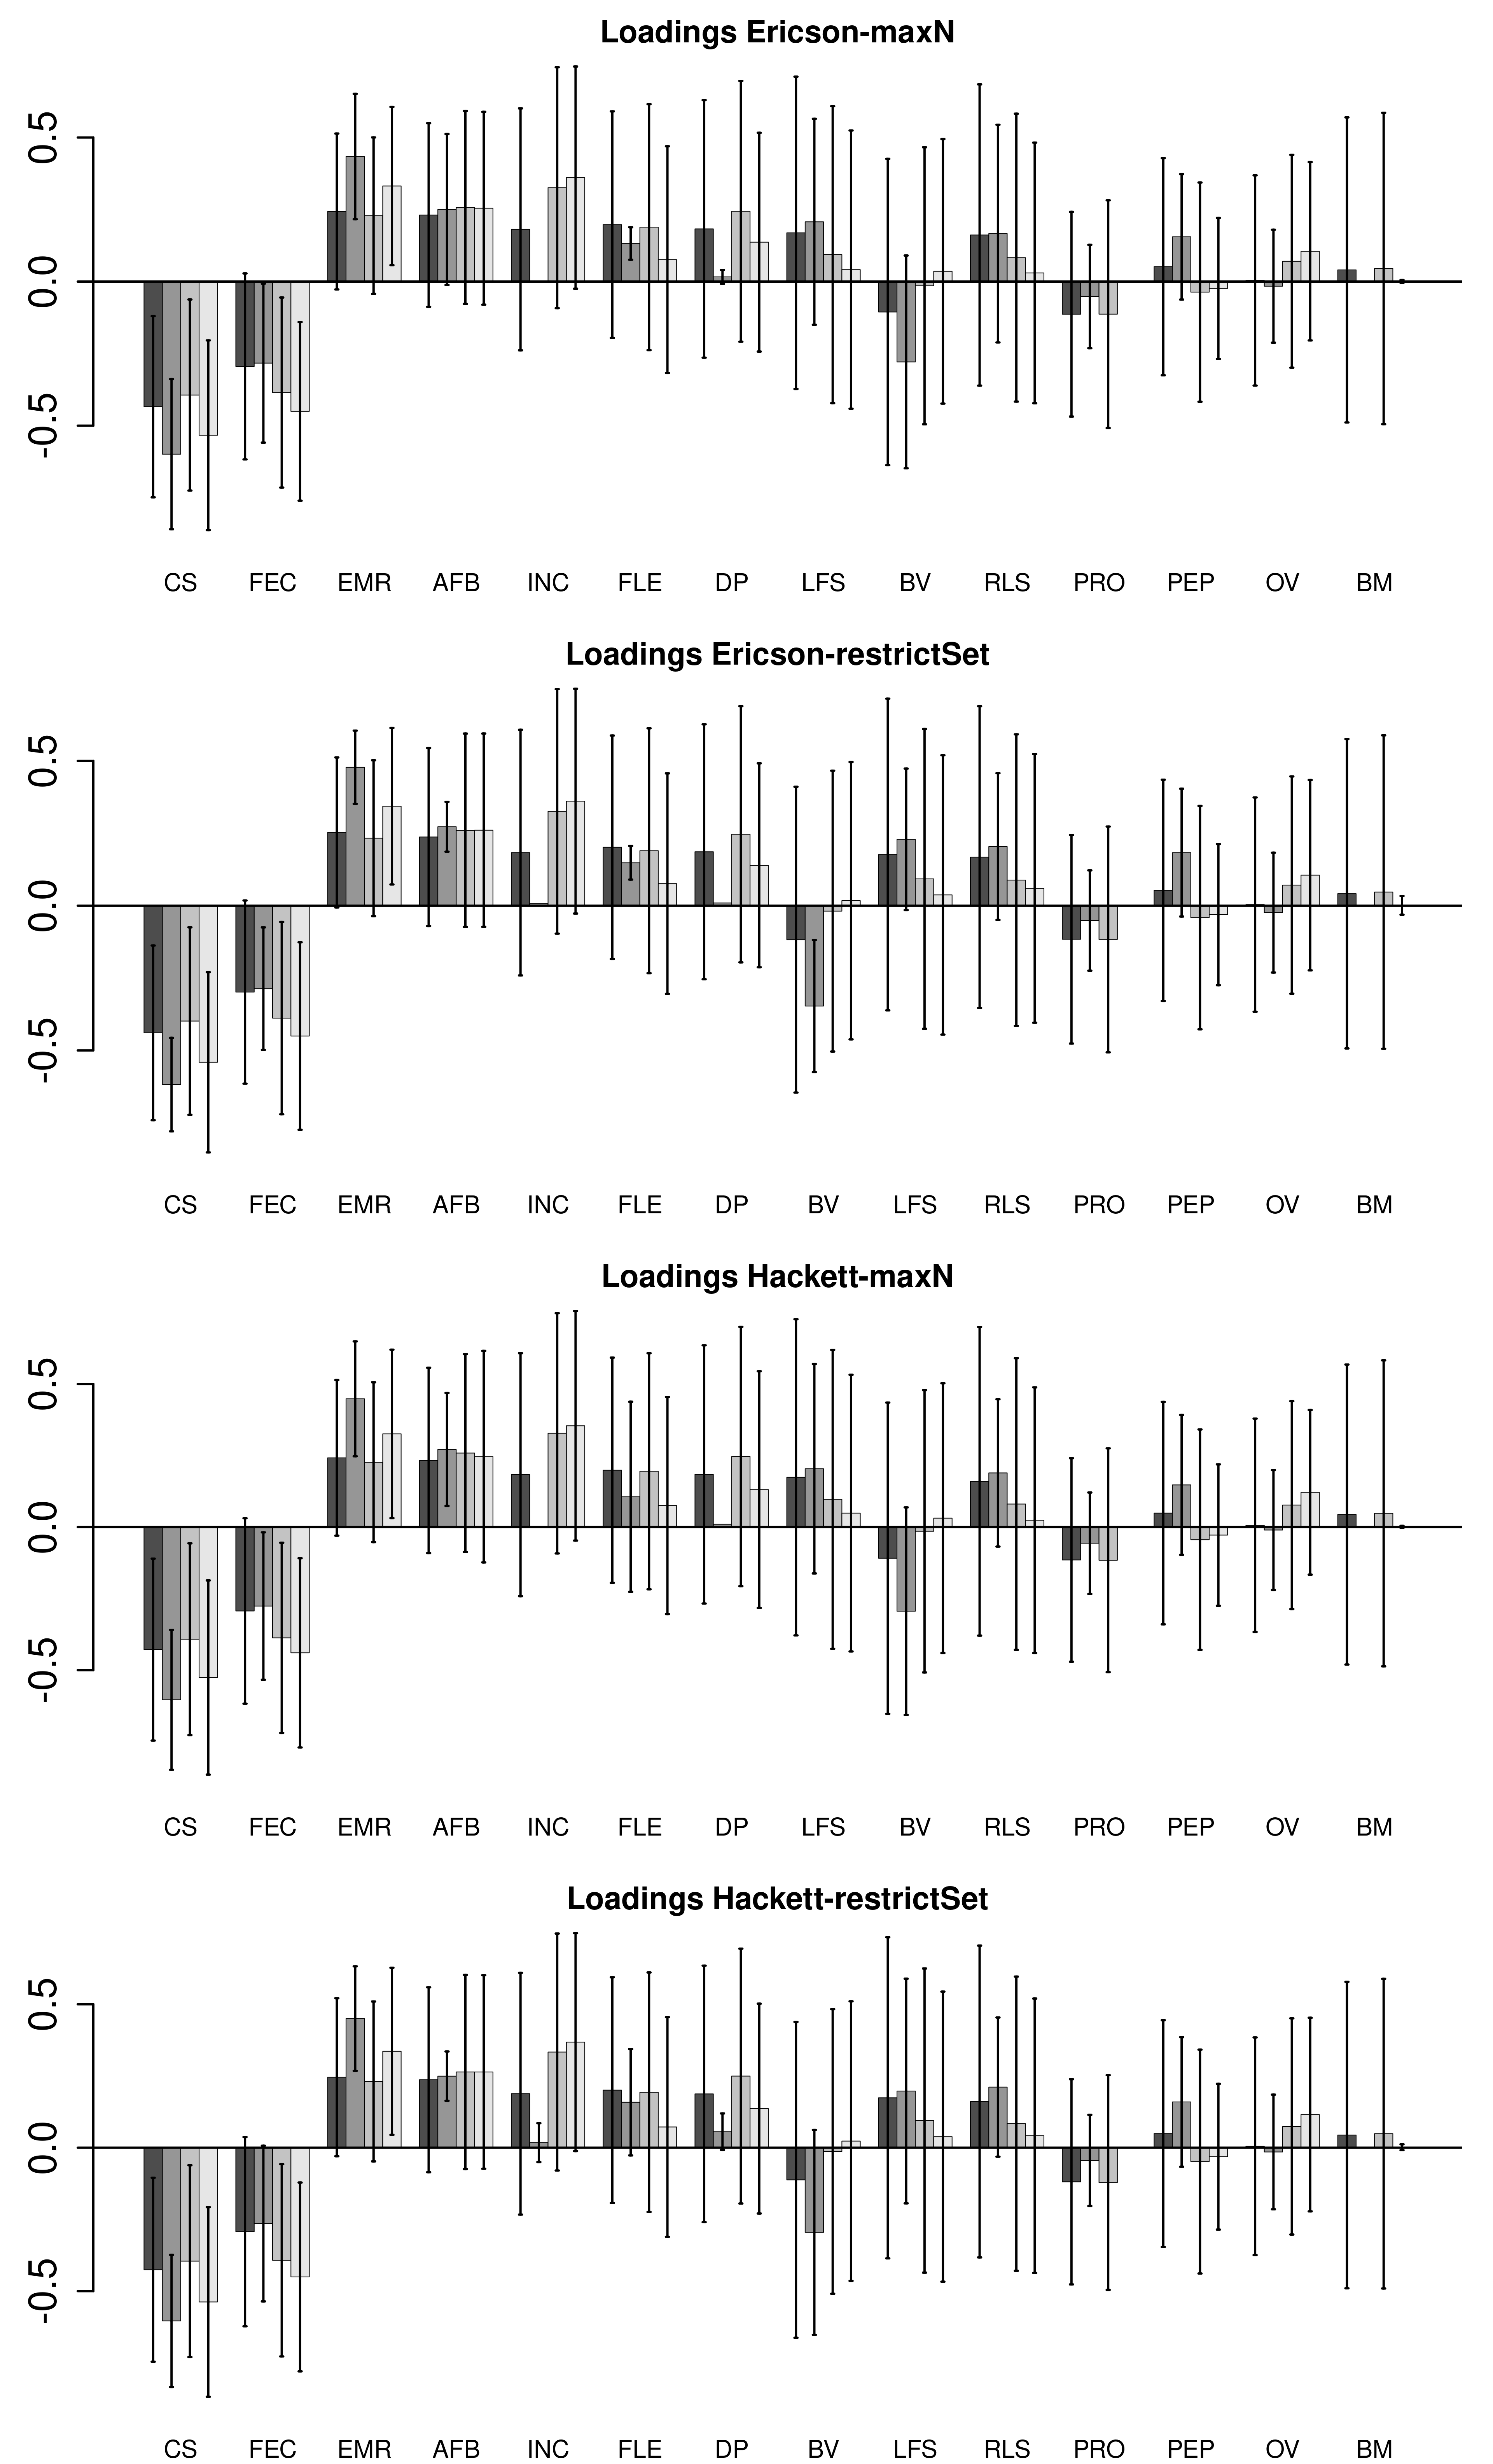
\includegraphics[width=.8\textwidth]{./Figures/Appendix2_1/FS loadings plots-ALL.png}
\caption[LHT loadings of the FS axes]{
Mean $\pm$ standard deviation AIC weighted loadings of the traits for the
fast-slow axes based on models predicting generation time or elasticity of
adult survival for all trait combination PCs o using only the PCs with AIC
\textless{2} (best AIC). From darker to lighter color: FSe, FSe best AIC, FSgt
and FSgt best AIC.}
\label{fig:figApp2.1}
\end{figure}

\begin{figure}[ht!]
\centering
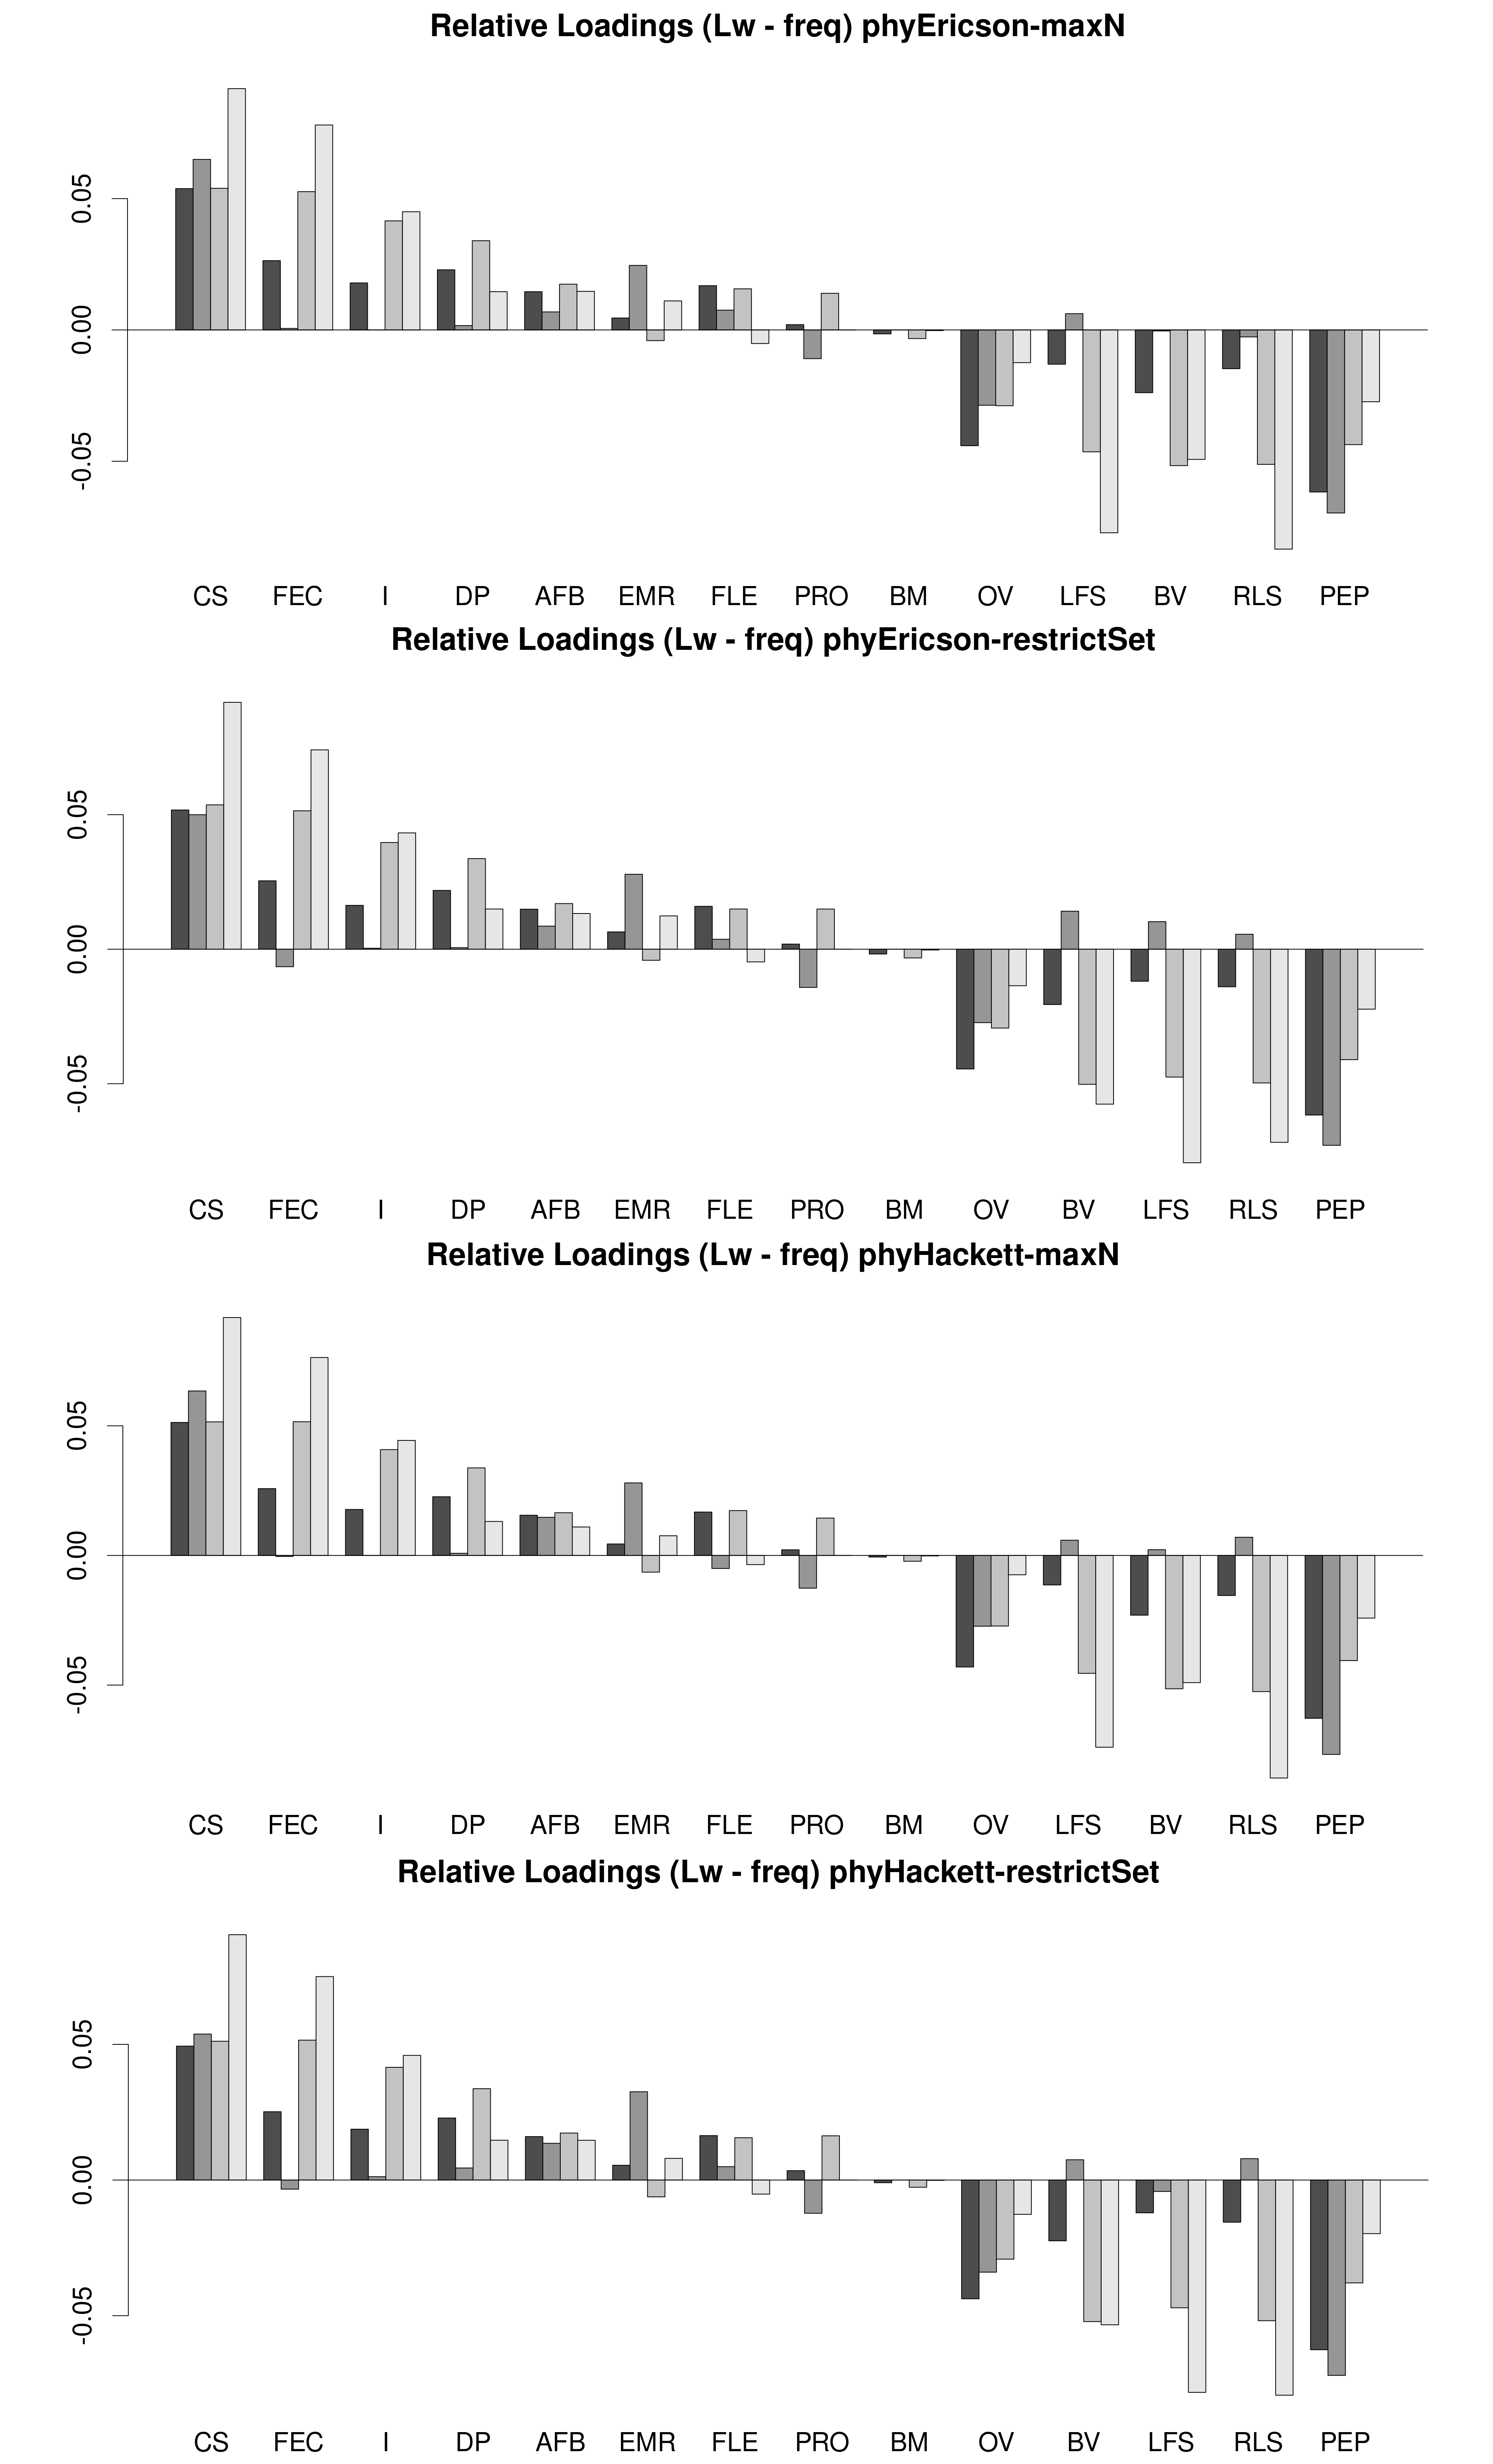
\includegraphics[width=.8\textwidth]{./Figures/Appendix2_1/FS relWeights plots-ALL.png}
\caption[LHT relative importance of the FS axes]{
Relative weight of the life history traits in the fast-slow continuum. Values
range from -1 to 1, where negative values means that the absolute value of the
trait loadings are lower than expected by the frequency of the trait and
positive values for traits with higher loadings than expected by the frequency
of the trait in the selected PPCAs (see main text for details). The loadings and
frequencies come from selected PCs that better predict elasticities of the
adult survival (FSe) or generation time (FSgt), weighted by the AIC based weight
of the models taking all or only the models with $\Delta AIC < 2$ (best AIC).
From darker to lighter color: FSe, FSe best AIC, FSgt and FSgt best AIC.}
\label{fig:figApp2.2}
\end{figure}

\begin{figure}[ht!]
\centering
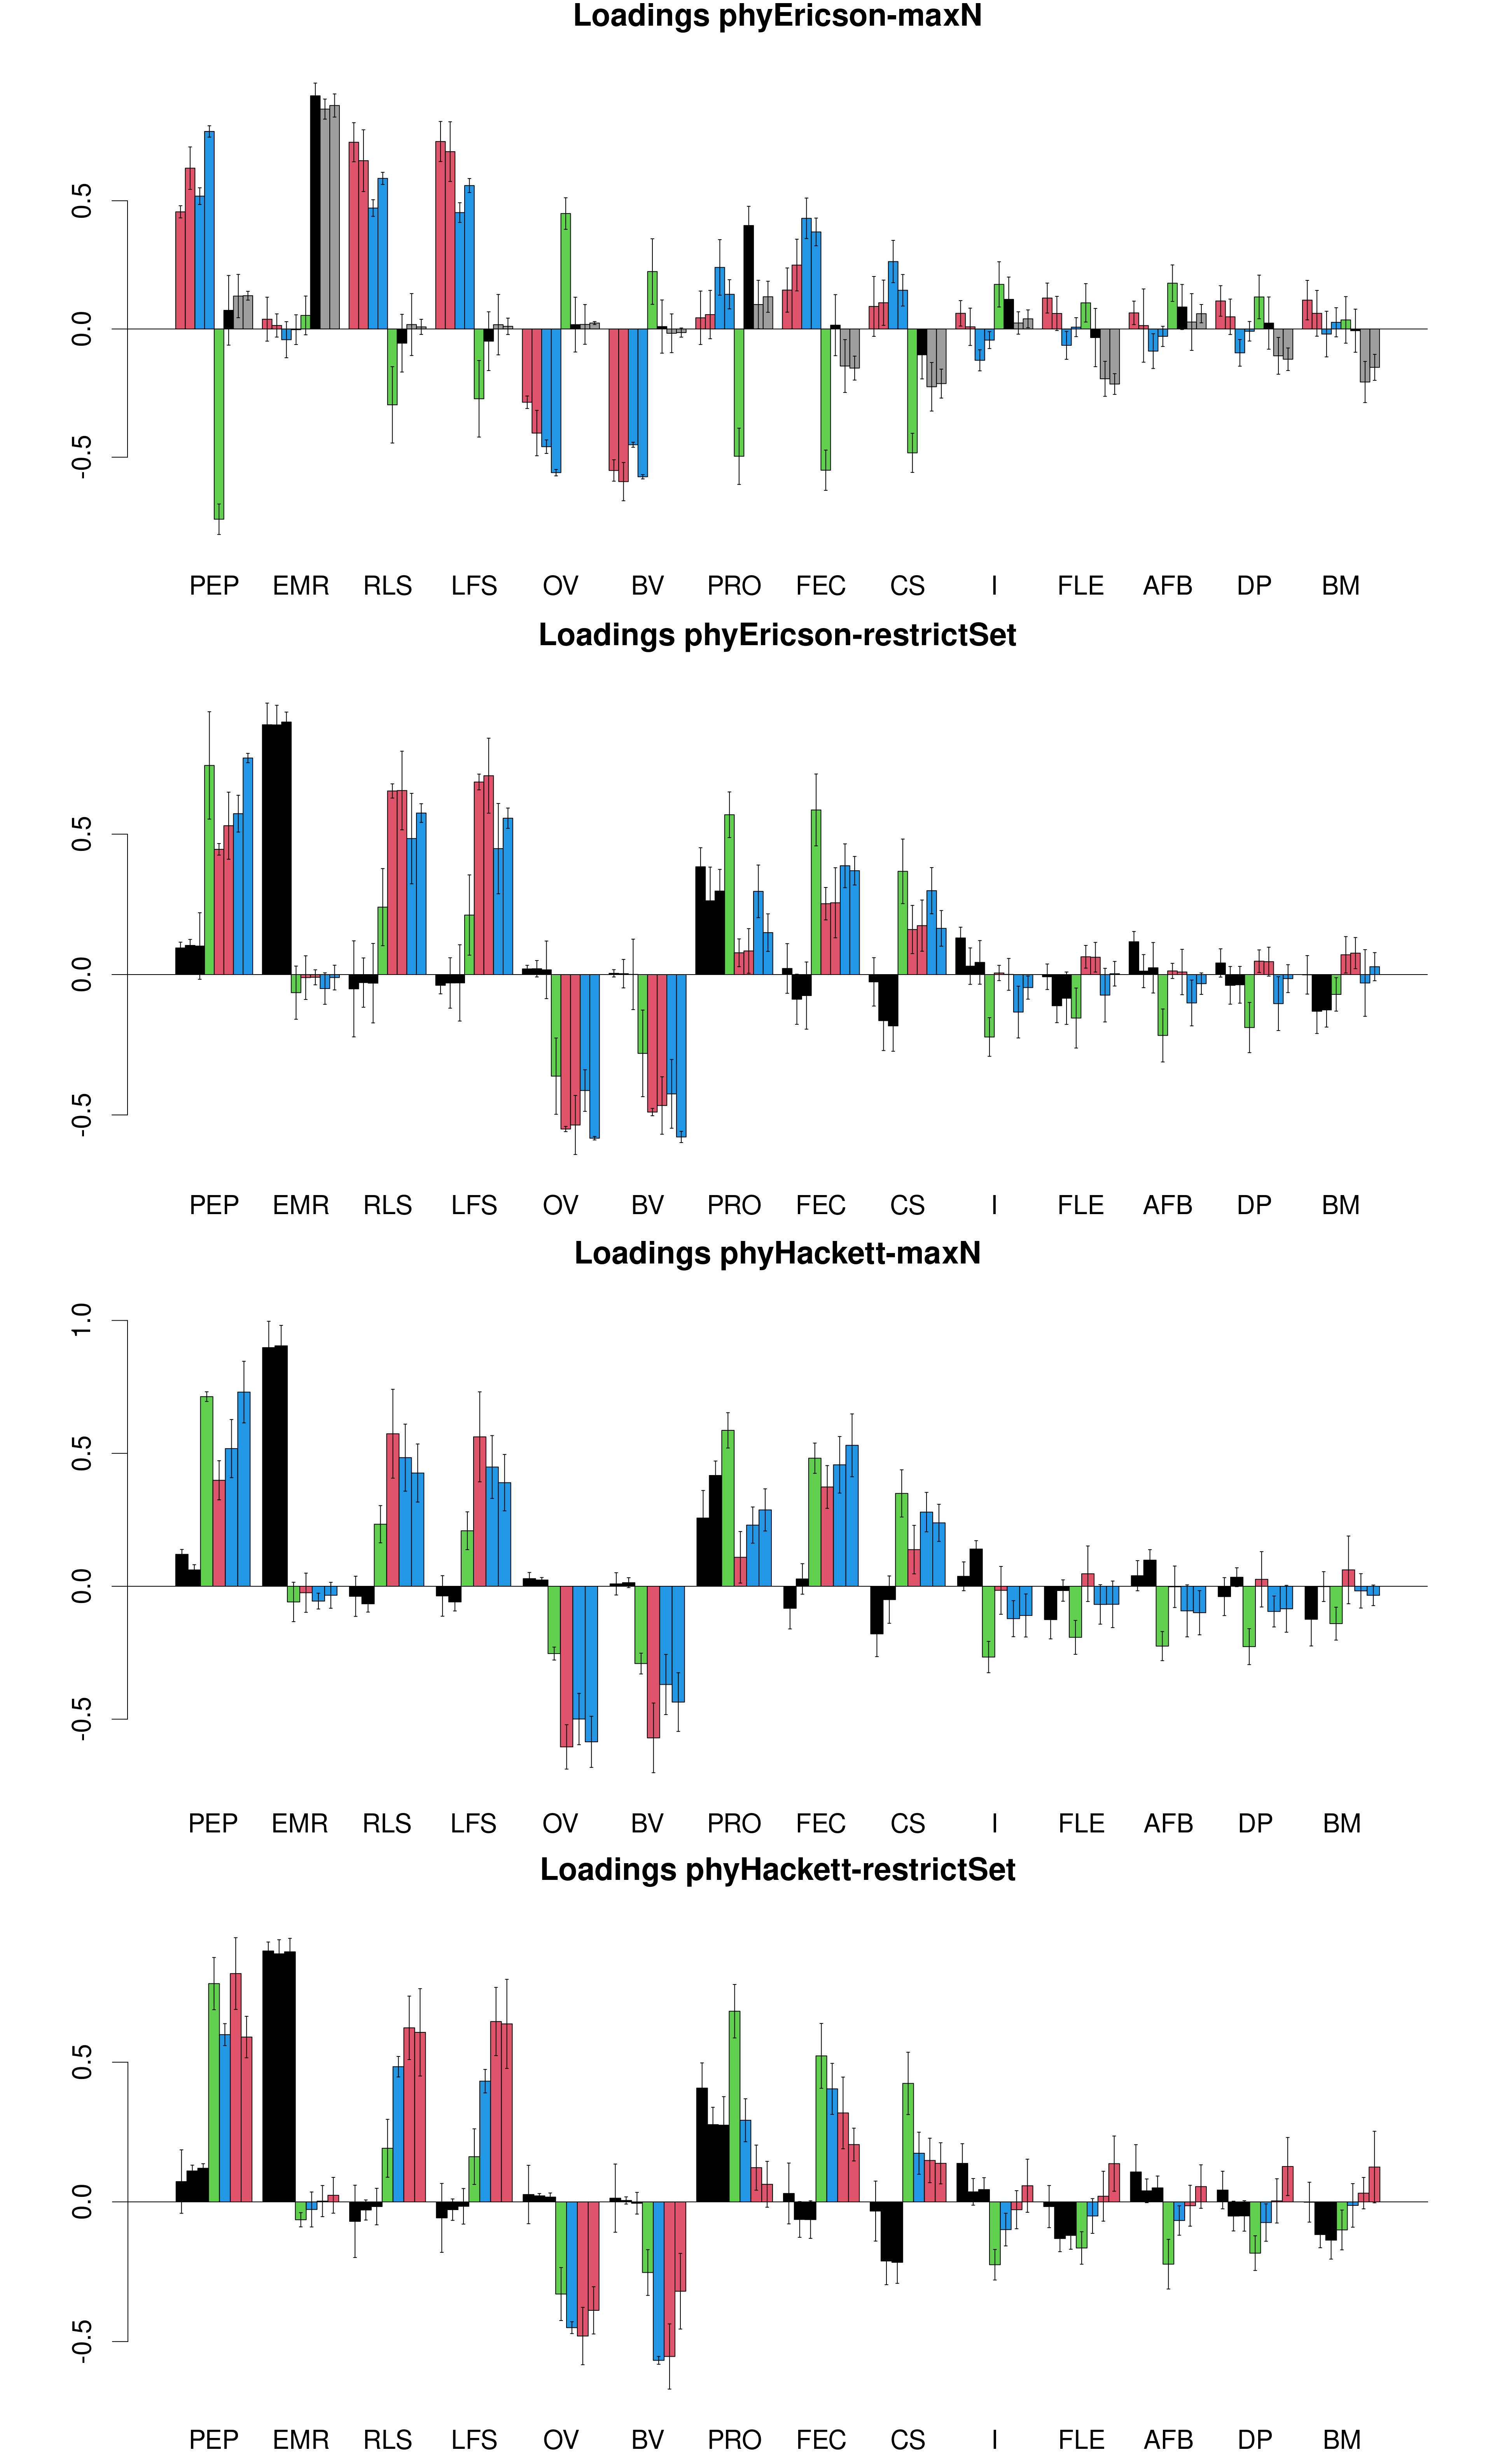
\includegraphics[width=.8\textwidth]{./Figures/Appendix2_1/2nd loadings plots-ALL.png}
\caption[LHT loadings of the secondary axes]{
Mean $\pm$ standard deviation of the loadings of the traits for clusters of
similar significant PCs (Eigenvalue \textgreater{1}) not selected for the
fast-slow axes. Groups follow the same order and colors than figure
\ref{fig:figApp2.5}.}
\label{fig:figApp2.3}
\end{figure}

\begin{figure}[ht!]
\centering
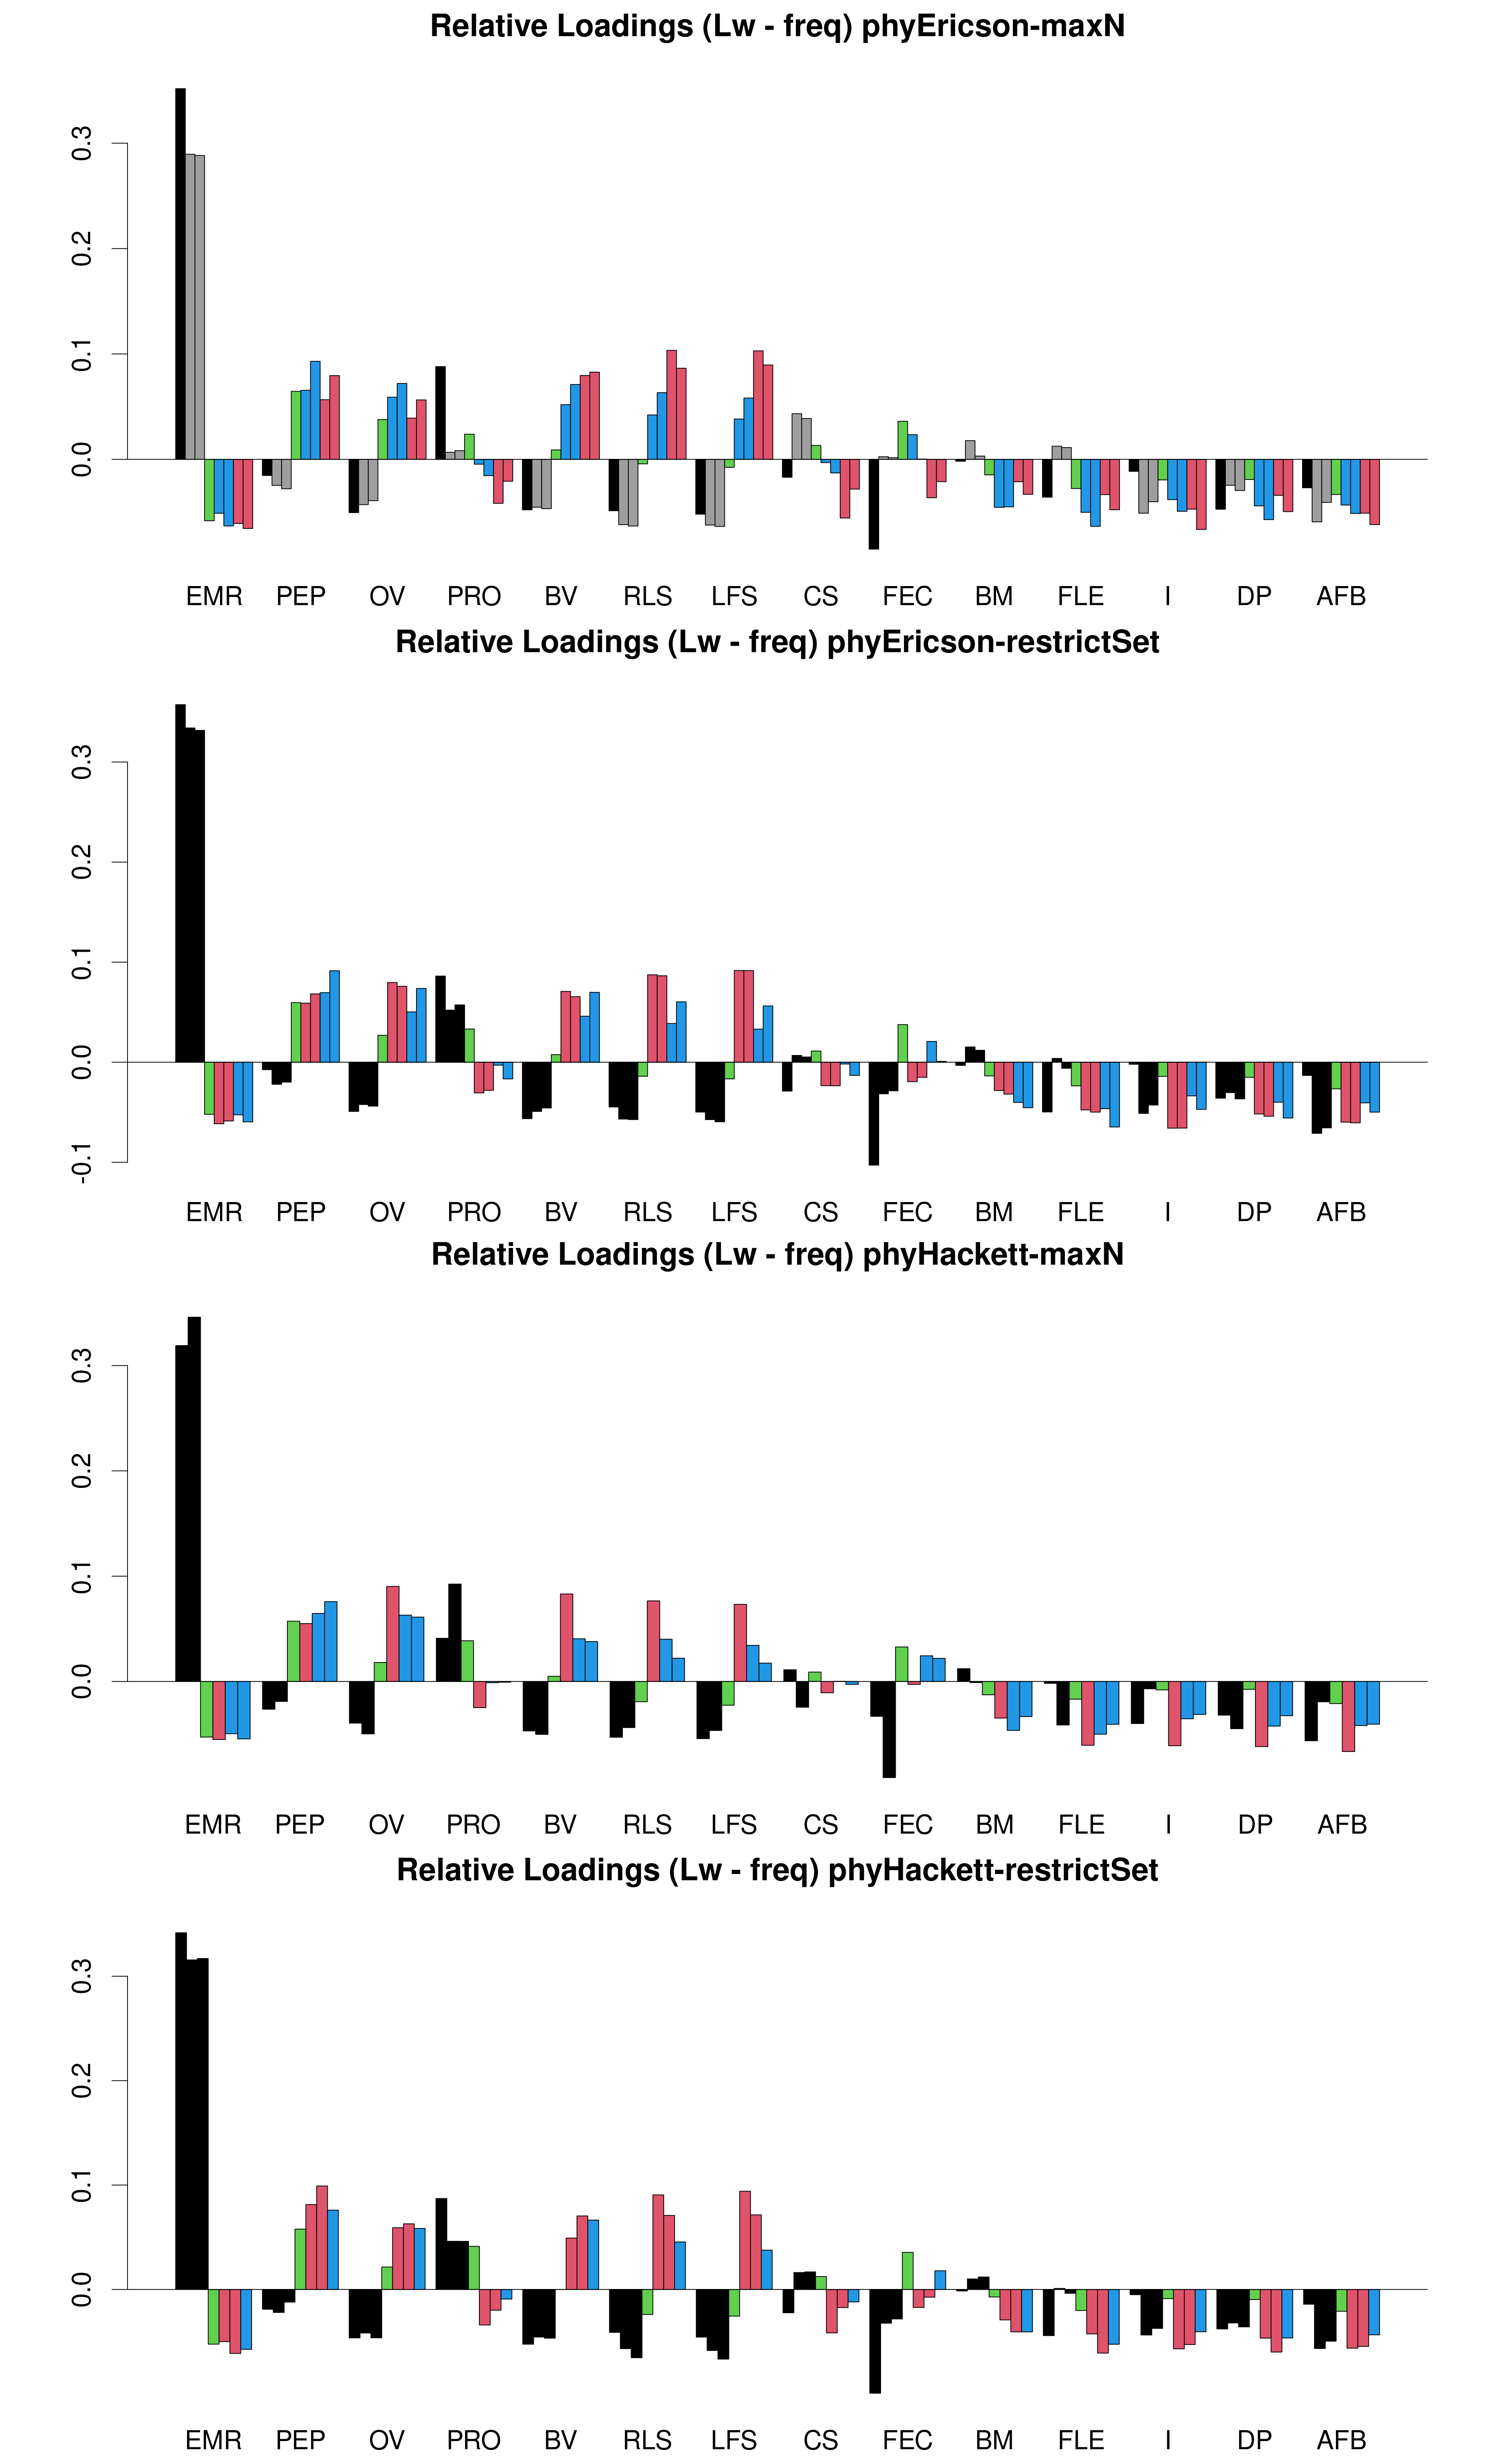
\includegraphics[width=.8\textwidth]{./Figures/Appendix2_1/2nd relWeights plots-ALL.png}
\caption[LHT relative importance of the secondary axes]{
Relative weights of the life history traits for each axes described in the
table \ref{tab:tabApp2.4}. Values range from -1 to 1, where negative values
means that the absolute value of the trait loadings are lower than expected by
the frequency of the trait and positive values for traits with higher loadings
than expected by the frequency of the trait in the selected PPCAs (see main
text for details). Groups follow the same order and colors than figure
\ref{fig:figApp2.5}.}
\label{fig:figApp2.4}
\end{figure}

\begin{figure}[ht!]
\centering
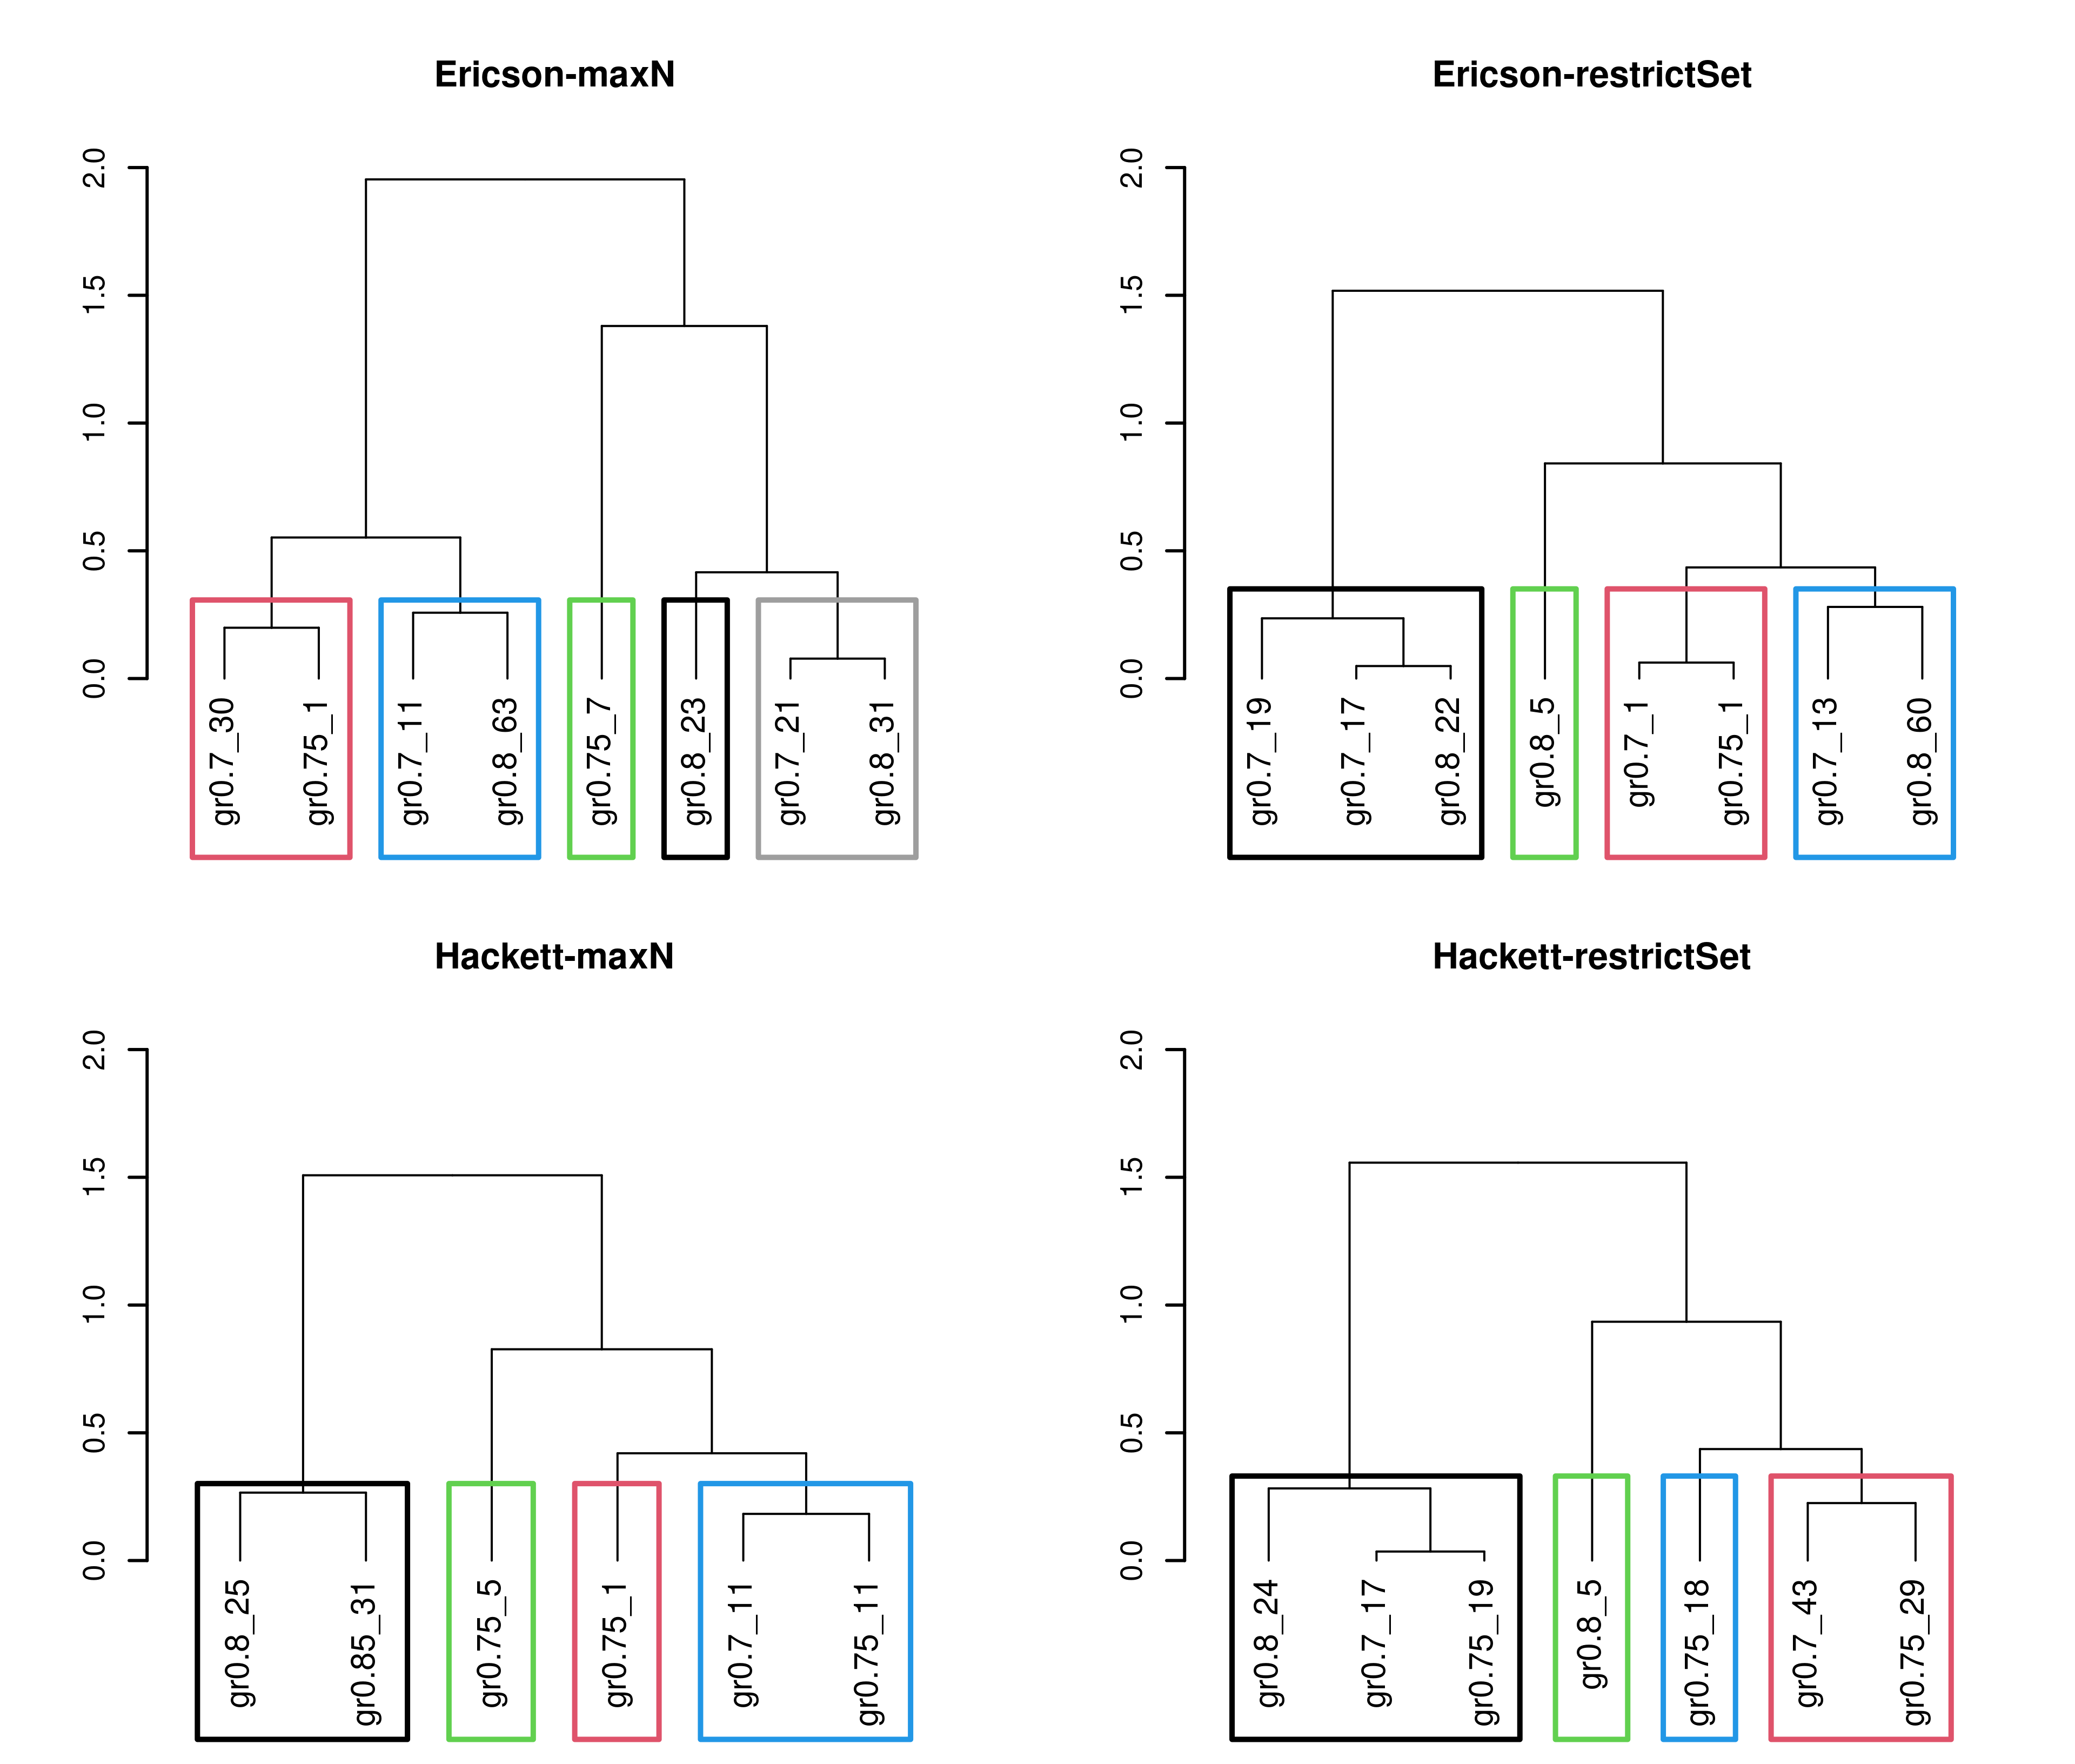
\includegraphics[width=.8\textwidth]{./Figures/Appendix2_1/2nd axes trees-1.png}
\caption[Cluster dendogram of the secondary axes]{
Dendogram of the distance among clusters of similar significant PCs (Eigenvalue
\textgreater{1}) not selected for the fast-slow axes. Each group contains PCs
with scores correlation greater than the correlation specified in the group name
(e.g. gr0.8 means correlation \textgreater{0.8}).}
\label{fig:figApp2.5}
\end{figure}
